\documentclass[11pt,a4paper]{article}

% Packages
\usepackage[utf8]{inputenc}
\usepackage[spanish, es-tabla]{babel}
\usepackage{caption}
\usepackage{listings}
\usepackage{adjustbox}
\usepackage{enumitem}
\usepackage{boldline}
\usepackage{amssymb, amsmath}
\usepackage[margin=1in]{geometry}
\usepackage{xcolor}
\usepackage{soul}
\usepackage{amsthm}  % insertar teoremas, corolarios...
\usepackage{multicol}
\usepackage{fancyhdr}
\pagestyle{fancy}
\lhead{\textbf{Relación de problemas Tema 1}}
\rhead{EDIP 1º DGIIM 2017/2018 · \textbf{Grupo 1}}
\cfoot{\thepage}
\renewcommand{\headrulewidth}{0.4pt}

\definecolor{grey}{RGB}{200, 200, 200}

% buscar entorno para proposiciones

\graphicspath{ {images/} }

% Meta
\title{%
  \textbf{Relación de problemas Tema 1} \\ Introducción a la Estadística Descriptiva unidimensional \\
  \hspace{1cm}\\
  \large \emph{Estadística Descriptiva e Introducción a la Probabilidad} \\
    1º DGIIM, 2017/2018}
\author{\small{Alumnos (\textbf{Grupo 1}):} \\
Miguel Ángel Fernández Gutiérrez \\
Eladia Gómez Morales \\
Marta Gómez Sánchez \\
Daniel Gonzálvez Alfert}
\date{\small{Fecha de entrega:} \\
\today}

% Custom
\providecommand{\abs}[1]{\lvert#1\rvert}
\setlength\parindent{0pt}
\definecolor{Light}{gray}{.90}
\newcommand\ddfrac[2]{\frac{\displaystyle #1}{\displaystyle #2}}

%Theorem envairoment
\newtheorem{theorem}{Teorema}[section]
\newtheorem{corollary}{Corolario}[theorem]


\theoremstyle{definition}
\newtheorem{definition}{Definición}[section]

\begin{document}
\maketitle

\hrulefill


%				##############################
%				#							 #
%				#  PROBLEMA 1				 #
%				#							 #
%				##############################


\begin{itemize}
	\item[\textbf{1.}] El número de hijos de las familias de una determinada barriada de una ciudad es una variable estadística de la que se conocen los siguientes datos:	



\begin{table}[htb]
\hspace*{2 cm}
\begin{tabular}{|c|c|c|c|c|}
$x_i$ & $n_i$ & $N_i$ & $f_i$ \\ \hline
0 & 80 & & 0.16 \\
1 & 110 & & \\
2 & & 320 & \\
3 & & & 0.18 \\
4 & 40 & & \\
5 & & & \\
6 & 20 & & \\ \hline
\end{tabular}
\hspace*{1.5cm}
{
\begin{tabular}{l}
$n_i$ : frecuencias absolutas \\
$N_i$ : frecuencias absolutas acumuladas \\
$f_i$ : frecuencias relativas
\end{tabular}}

\end{table}

	\begin{itemize}
		\item[\emph{a)}] Completar la tabla de frecuencias.
		\item[\emph{b)}] Representar la distribución mediante un diagrama de barras y la curva de distribución.
		\item[\emph{c)}] Promediar los valores de la variable mediante diferentes medidas. Interpretarlas.
	\end{itemize}
\end{itemize}

{\color{grey}\hrulefill}

\emph{Solución:} \\

Antes de nada, caracterizaremos nuestro \emph{puñetero asterisco}:

\begin{itemize}
	\item[$\circledast$] \textbf{Población:} las familias de una determinada barriada ($n=500$). \\ \textbf{Variable estadística:} el número de hijos de cada una de las familias. \\ \textbf{Número de modalidades:} $k=7$
\end{itemize}

\small{\textbf{Nota:} caracterizaremos nuestro \emph{puñetero asterisco} al principio de cada uno de los problemas.}

\pagebreak

Dicho esto, procederemos a hacer cada uno de los apartados del problema:

\begin{itemize}
	\item[\emph{a)}] La tabla completa es la siguiente:
\end{itemize}



\begin{table}[!htbp]
\hspace*{2 cm}
\begin{tabular}{|c|c|c|c|c|c|}
$x_i$ & $n_i$ & $N_i$ & $f_i$ & $x_in_i$ \\ \hline
0 & 80 & 80 & 0.16 & 0 \\
1 & 110 & 190 & 0.22 & 110 \\
2 & 130 & 320 & 0.26 & 260  \\
3 & 90 & 410 & 0.18 & 270\\
4 & 40 & 450 & 0.08 & 160 \\
5 & 30 & 480 & 0.06 & 150\\
6 & 20 & 500 & 0.04 & 120 \\ \hline
\multicolumn{1}{c}{} & \multicolumn{1}{|c|}{500} & \multicolumn{1}{c}{} & \multicolumn{1}{c}{} & \multicolumn{1}{|c|}{1070} \\ \cline{2-2} \cline{5-5}
\end{tabular}
\hspace*{1cm}
{
\begin{tabular}{l}
$n_i$ : frecuencias absolutas \\
$N_i$ : frecuencias absolutas acumuladas \\
$f_i$ : frecuencias relativas \\
\\
\small{\textbf{Nota:} de ahora en adelante, insertaremos en} \\
\small{las tablas las columnas necesarias para realizar} \\
\small{los cálculos pertintentes al problema.}
\end{tabular}}

\end{table}



\begin{itemize}
	\item[\emph{b)}] Las gráficas son las siguientes: \\

\hspace{0.5cm} 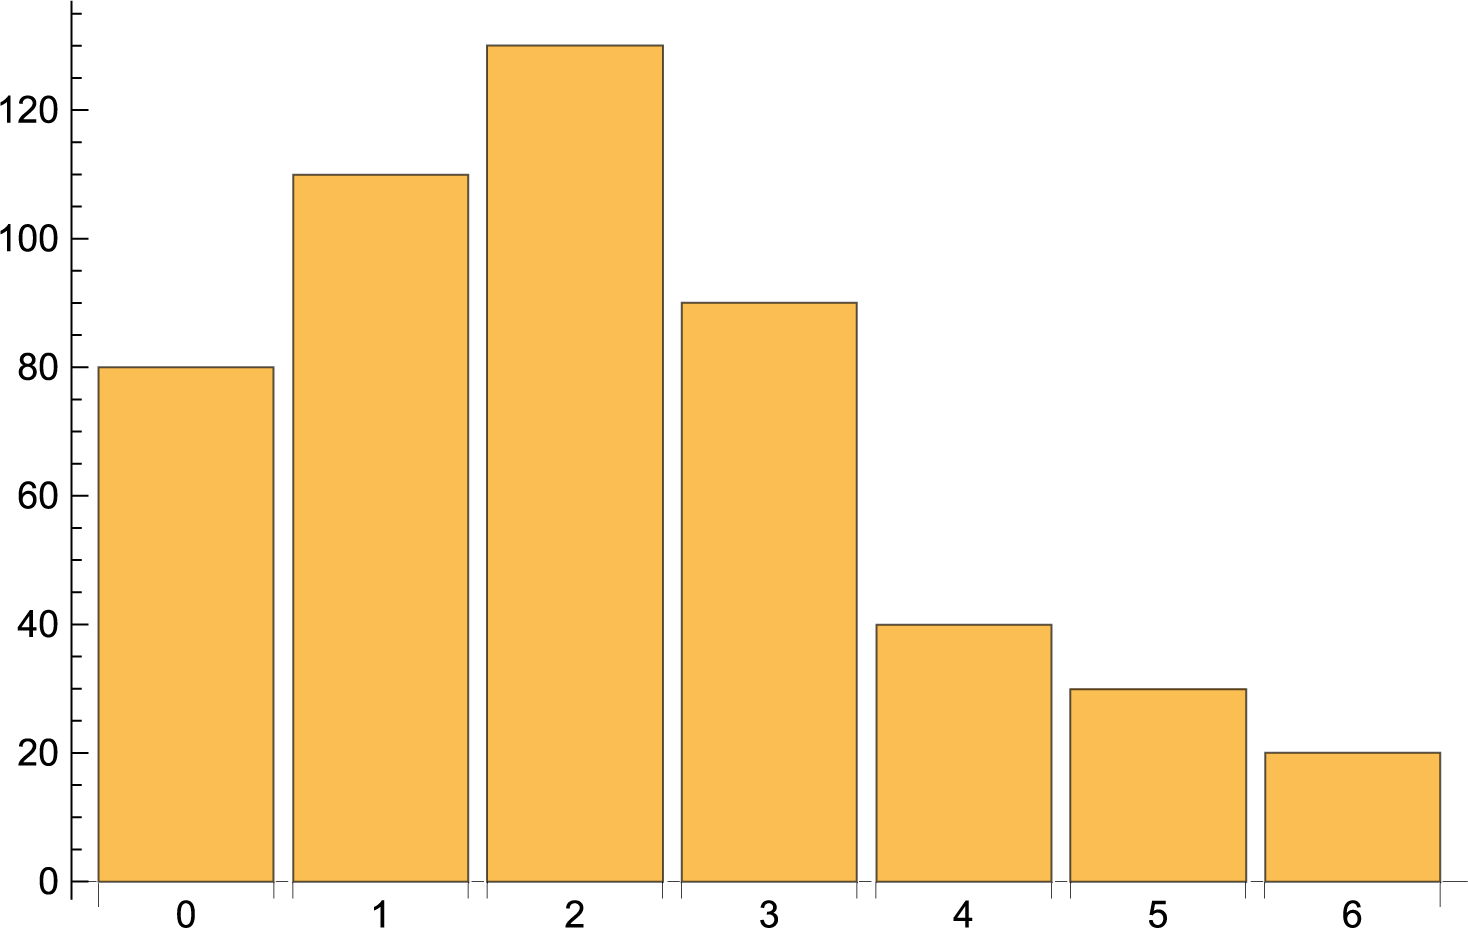
\includegraphics[width=6.5cm]{ej1_barr.png} \hspace{0.5cm} 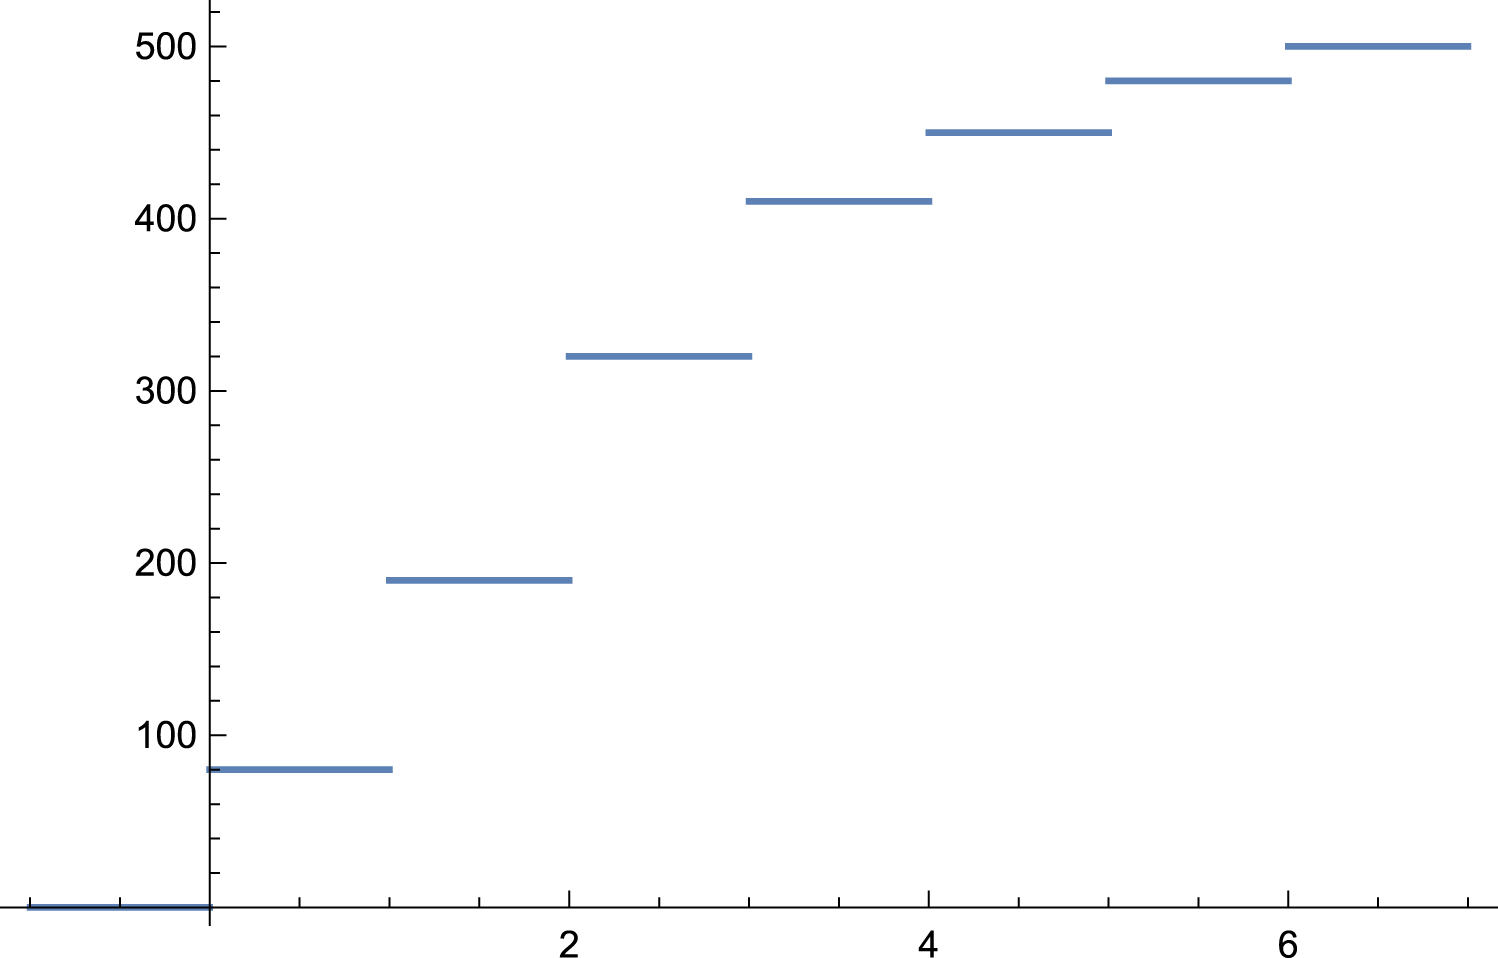
\includegraphics[width=6.5cm]{ej1_curva.png}

\begin{multicols}{2}
\begin{center}
\small{Gráfica de barras} \\
\end{center}
\begin{center}
\small{Curva de distribución}
\end{center}
\end{multicols}

	\item[\emph{c)}] Lo promediaremos con las siguientes medidas estadísticas:
	\begin{itemize}
		\item \textbf{Media:} usamos la \textbf{media aritmética}. 
		$$ \bar{x} = \frac{1}{n} \sum_{i=1}^{k}x_{i}n_{i}= 2.14 $$
		El valor es representativo de los datos, pues se trata de una variable unidimensional, que no es acumulativa ni depende del cociente de otras dos magnitudes.
		\item[] \emph{Por lo expuesto anteriormente, el resto de medidas de posición (media armónica y media geométrica) no tienen sentido en este caso.}
		\item \textbf{Mediana: } $Me = 2$, puesto que $n/2=250 < N_3$, y $Me = x_3 = 2$.
		\item[] La mitad de las familias tienen dos o menos hijos.
		\item \textbf{Moda: } $Mo = 2$, que es la variable con mayor $n_i$.
		\item[] La mayoría de las familias tienen dos hijos.
	\end{itemize}
\end{itemize}


%				##############################
%				#							 #
%				#  PROBLEMA 2				 #
%				#							 #
%				##############################


\pagebreak

\begin{itemize}
	\item[\textbf{2.}] La puntuación obtenida por 50 personas que se presentaron a una prueba de selección, sumadas las puntuaciones de los distintos tests, fueron:
	\center{174, 185, 166, 176, 145, 166, 191, 175, 158, 156, 156, 187, 162, 172, 197, 181, 151,\\
161, 183, 172, 162, 147, 178, 176, 141, 170, 171, 158, 184, 173, 169, 162, 172, 181,\\
187, 177, 164, 171, 193, 183, 173, 179, 188, 179, 167, 178, 180, 168, 148, 173.}

	\begin{itemize}
		\item[\emph{a)}] Agrupar los datos en intervalos de amplitud 5 desde 140 a 200 y dar la tabla de frecuencias.
		\item[\emph{b)}] Representar la distribución mediante un histograma, poligonal de frecuencias y curva de distribución.
	\end{itemize}
\end{itemize}

{\color{grey}\hrulefill}

\emph{Solución:}

\begin{itemize}
	\item[$\circledast$] \textbf{Población:} las familias de una determinada barriada. \\ \textbf{Variable estadística:} el número de hijos de cada una de las familias ($n=50$). \\ \textbf{Número de modalidades: } $k=12$.
\end{itemize}

\begin{itemize}
	\item[\emph{a)}] La tabla completa es la siguiente:

\begin{table}[!htbp]
\hspace*{2 cm}
\begin{tabular}{|c|c|c|c|c|c|c|c|}
\multicolumn{1}{c|}{$I_i$} & $n_i$ & $N_i$ & $f_i$ & $F_i$ & $c_i$ & $a_i$ & $h_i$ \\ \hline
$[140, 145]$ &  2	&  2	& 0.04	& 0.04 & 142.5 & 5 & 0.008 \\
$(145, 150]$ &  2	&  4	& 0.04	& 0.08	& 147.5	& 5 & 0.008\\
$(150, 155]$ &  1	&  5	& 0.02	& 0.1	& 152.5	& 5 & 0.004\\
$(155, 160]$ &  4	&  9	& 0.08	& 0.18	& 157.5	& 5 & 0.016\\
$(160, 165]$ &  5	& 14	& 0.1	& 0.28	& 162.5	& 5 & 0.02\\
$(165, 170]$ &  6	& 20	& 0.12	& 0.4	& 167.5 & 5 & 0.024	\\
$(170, 175]$ & 10	& 30	& 0.2	& 0.6 & 172.5 & 5 & 0.04 \\
$(175, 180]$ &  8	& 38	& 0.16	& 0.76 & 177.5 & 5 & 0.032 \\
$(180, 185]$ &  6	& 44	& 0.12	& 0.88 & 182.5 & 5 & 0.024 \\
$(185, 190]$ &  3	& 47	& 0.06	& 0.94 & 187.5 & 5 & 0.012 \\
$(190, 195]$ &  2	& 49	& 0.04	& 0.98 & 192.5 & 5 & 0.008 \\
$(195, 200]$ &  1	& 50	& 0.02	& 1 & 197.5 & 5 & 0.004 \\ \hline
\multicolumn{1}{c}{} & \multicolumn{1}{|c|}{50} & \multicolumn{1}{c}{} & \multicolumn{1}{c}{} & \multicolumn{1}{c}{} \\ \cline{2-2}
\end{tabular}
\end{table}

	\item[\emph{b)}] Las gráficas son las siguientes: \\
	
	
\hspace{0.5cm} 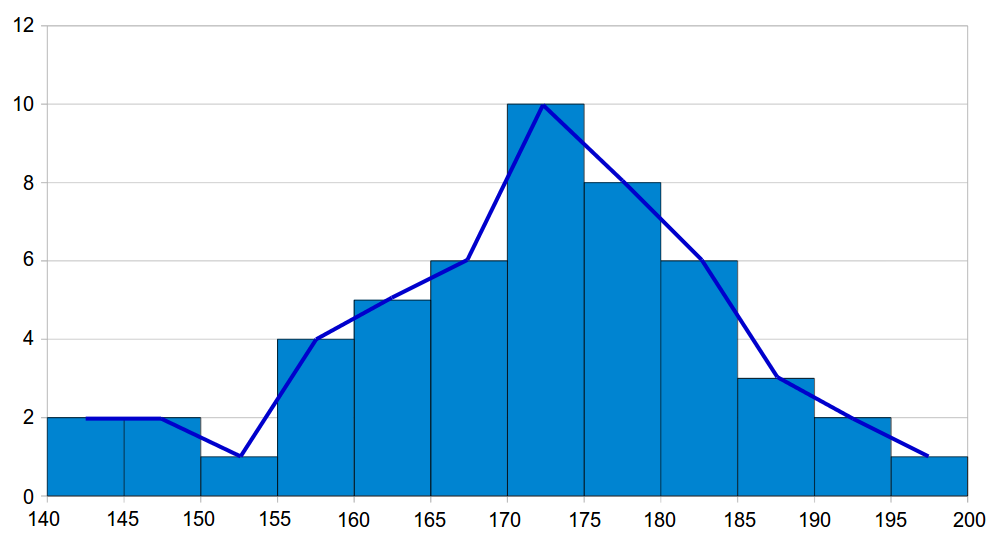
\includegraphics[width=6.5cm]{ej2_hist.png} \hspace{0.5cm} 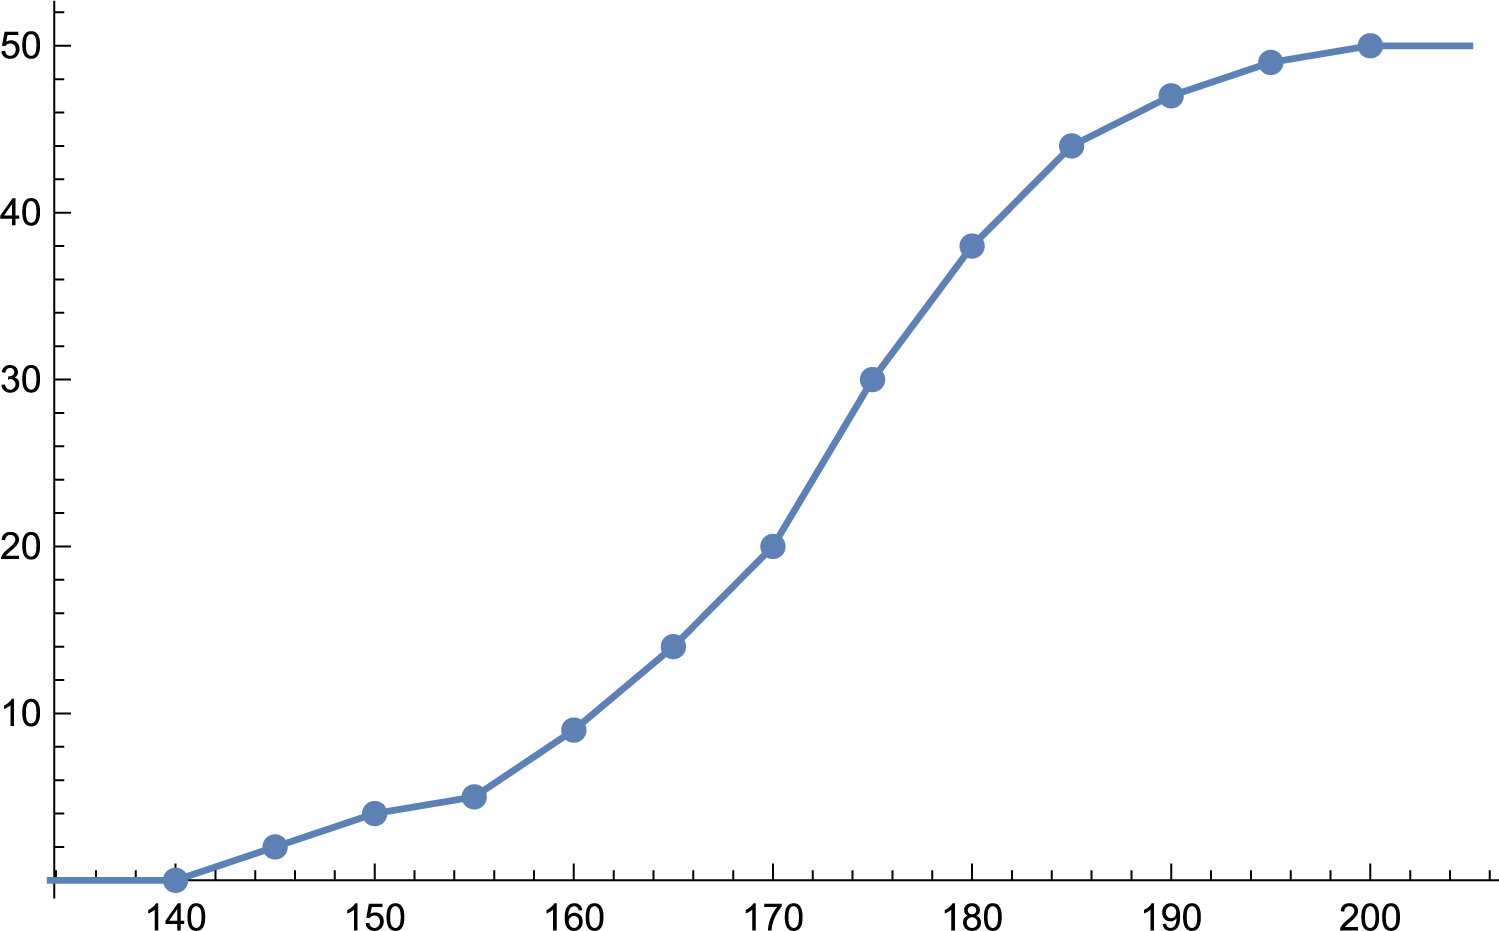
\includegraphics[width=6.5cm]{ej2_curva.png}

\begin{multicols}{2}
\begin{center}
\small{Histograma y poligonal de frecuencias} \\
\end{center}
\begin{center}
\small{Curva de distribución}
\end{center}
\end{multicols}
\end{itemize}
\hspace{2cm} \\



%				##############################
%				#							 #
%				#  PROBLEMA 3				 #
%				#							 #
%				##############################


\pagebreak

\begin{itemize}
	\item[\textbf{3.}] La distribución de la renta familiar en el año 2003 por comunidades autónomas se recoge en la siguiente tabla:


\begin{table}[!htbp]
\begin{tabular}{|c|c|c|c|c|c|c|c|}
\multicolumn{1}{c|}{$I_i$} & $n_i$ & $N_i$ & $f_i$ & $F_i$ & $c_i$ & $a_i$ & $h_i$ \\ \hline
$(8300, 9300]$				& 2	& 		& 		& 		& 		& 		&  \\
$(\hspace{0.6cm}, 10200]$	& 	& 5		& 		& 		& 		& 		&  \\
							&	& 		& 		& 10/18	& 		& 1100	&  \\
							& 	& 		& 2/18	& 		& 12000	& 		&  \\
							& 4	& 		& 		& 		& 		& 		& 0.005/18 \\
							& 	& 18	&		& 		& 		& 		& 0.002/18 \\ \hline
\end{tabular}
\hspace*{0.2cm}
{
\begin{tabular}{l}
$n_i$ : frecuencias absolutas \\
$N_i$ : frec. abs. acumuladas  \\
$f_i$ : frecuencias relativas \\
$F_i$ : frec. rel. acumuladas \\
$c_i$ : marcas de clase \\
$a_i$ : amplitudes \\
$h_i$ : densidades de frecuencia
\end{tabular}}

\end{table}


	\begin{itemize}
		\item[\emph{a)}] Completar la tabla.
		\item[\emph{b)}] Representar la distribución mediante un histograma, poligonal de frecuencias y curva de distribución.
		\item[\emph{c)}] ¿Cuántas comunidades presentan una renta menor o igual que 12700 euros? ¿Y cuántas superior a 11300 euros?
	\end{itemize}
\end{itemize}

{\color{grey}\hrulefill}

\emph{Solución:}

\begin{itemize}
	\item[$\circledast$] \textbf{Población:} las comunidades autónomas de España, contando a Ceuta y Melilla como una ($n=18$). \\ \textbf{Variable estadística:} la renta familiar.
	\item[\emph{a)}] La tabla completa es:

\begin{table}[!htbp]
\hspace{2cm}
\begin{tabular}{|c|c|c|c|c|c|c|c|}
\multicolumn{1}{c|}{$I_i$} & $n_i$ & $N_i$ & $f_i$ & $F_i$ & $c_i$ & $a_i$ & $h_i$ \\ \hline
$(8300, 9300]$ & 2	& 	2	& 2/18 & 2/18 & 8800 & 	1000	&  0.002/18\\
$(9300, 10200]$ & 3 & 5		& 3/18 & 5/18 & 9750 & 	900	& 0.003/18 \\
$(10200, 11300]$ & 5 & 	10	& 5/18 & 10/18	& 10750 & 1100	& 0.05/18  \\
$(11300, 12700]$ & 2 & 	12	& 2/18	& 12/18 & 12000	& 	1400	& 0.002/18 \\
$(12700, 13500]$ & 4	& 16	& 	4/18	& 	16/18	& 13100		& 	800	& 0.005/18 \\
$(13500, 14500]$ & 2	& 18	&	2/18	& 1		& 	14000	& 	1000	& 0.002/18 \\ \hline
\end{tabular}
\end{table}
	\item[\emph{b)}] Las gráficas son las siguientes: \\

\hspace{0.5cm} 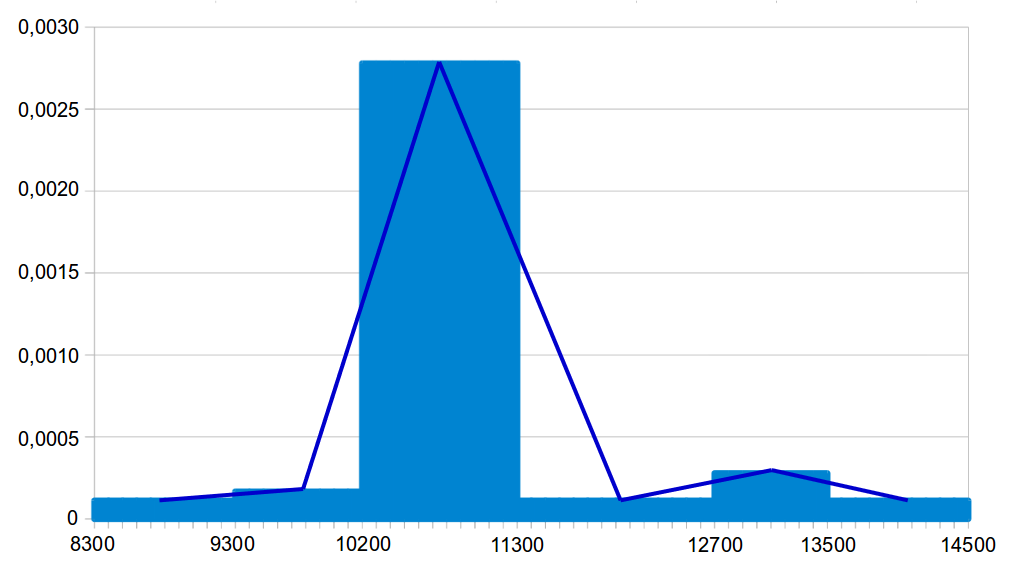
\includegraphics[width=6.5cm]{ej3_hist.png} \hspace{0.5cm} 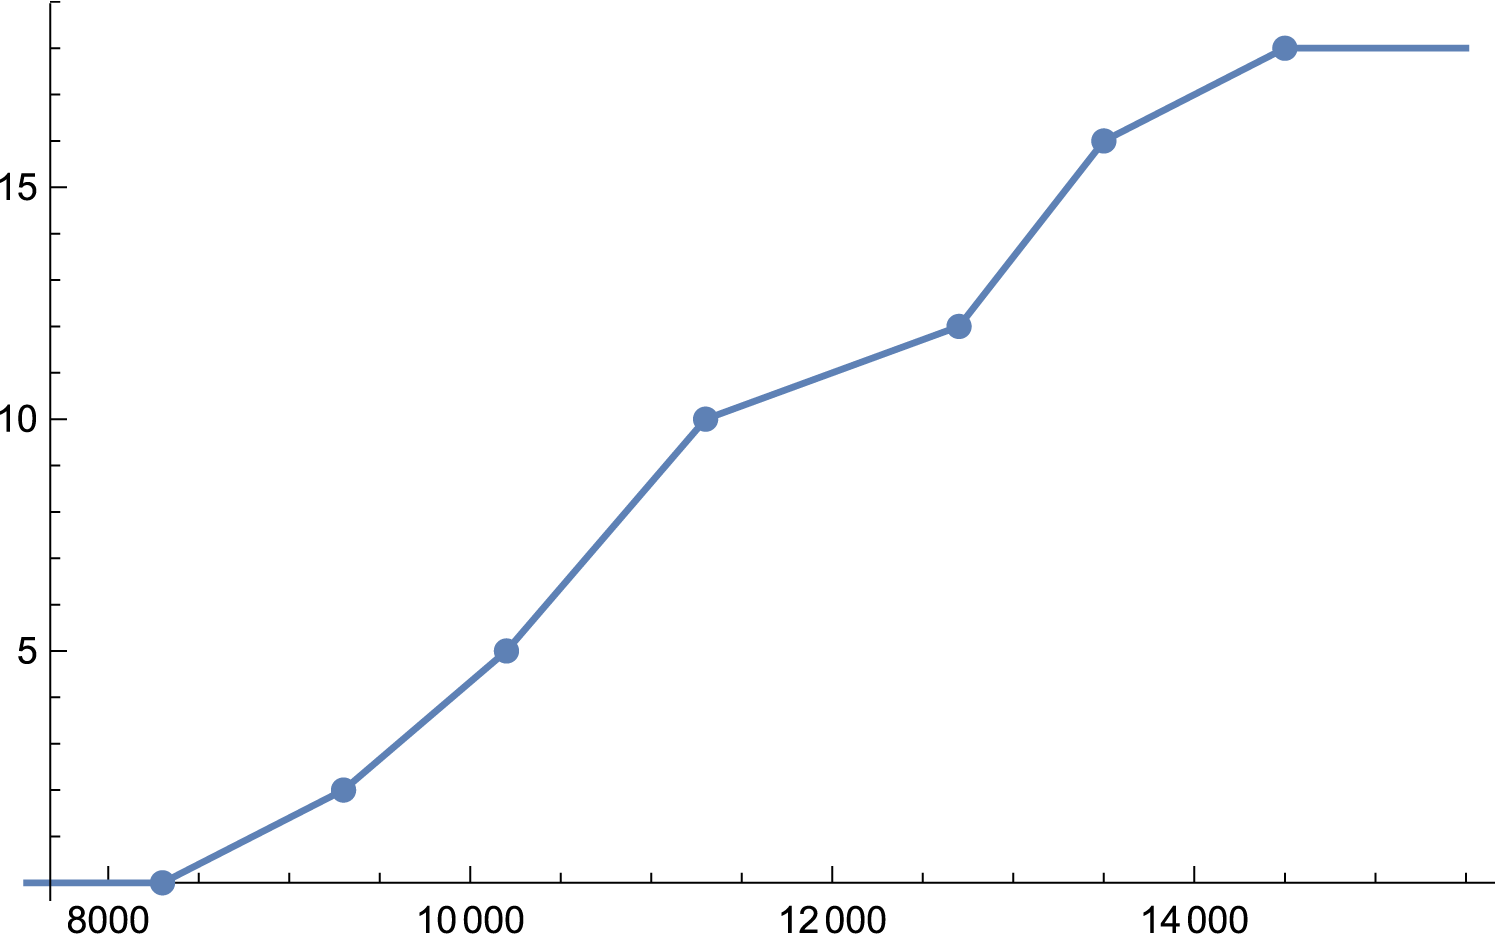
\includegraphics[width=6.5cm]{ej3_curva.png}

\begin{multicols}{2}
\begin{center}
\small{Histograma y poligonal de frecuencias} \\
\end{center}
\begin{center}
\small{Curva de distribución}
\end{center}
\end{multicols}
	\item[\emph{c)}] 12 comunidades presentan una renta menor o igual que 12700 euros (simplemente $N_4$ = 12). \\
	8 comunidades presentan una renta superior a 11300 euros (basta calcular $n-N_3=18-10=8$, puesto que al ser las comunidades que presentan una renta superior a 11300, la cota inferior de $I_4$, debemos de contar también el $n_4$, y $n_4 + n_5 + n_6 = n - N_3$).

\end{itemize}


%				##############################
%				#							 #
%				#  PROBLEMA 4				 #
%				#							 #
%				##############################


\pagebreak

\begin{itemize}
	\item[\textbf{4.}] En una determinada empresa se realiza un estudio sobre la calidad de su producción. La distribución siguiente informa sobre el número de piezas defectuosas encontradas en 100 cajas
examinadas con 50 unidades cada una de ellas:


\begin{table}[!htbp]
\hspace{2cm}
\begin{tabular}{|c|||c|c|c|c|c|c|c|c|c|c|c|}
\hline
Nº piezas defectuosas & 0 & 1 & 2 & 3 & 4 & 5 & 6 & 7 & 8 & 9 & 10 \\ \hline
Nº de cajas			  & 6 & 9 & 10 & 11 & 14 & 16 & 16 & 9 & 4 & 3 & 2 \\ \hline
\end{tabular}
\end{table}
	\begin{itemize}
		\item[\emph{a)}] Calcular el número medio de piezas defectuosas por caja.
		\item[\emph{b)}] ¿Cuántas piezas defectuosas se encuentran más frecuentemente en las cajas examinadas?
		\item[\emph{c)}] ¿Cuál es el número mediano de piezas defectuosas por caja?
		\item[\emph{d)}] Calcular los cuartiles de la distribución. Interpretarlos.
		\item[\emph{e)}] Calcular los deciles de orden 3 y 7. Interpretarlos.
		\item[\emph{f)}] Cuantificar la dispersión de la distribución utilizando diferentes medidas, interpretando los resultados y señalando las ventajas e inconvenientes de cada una.
	\end{itemize}
\end{itemize}

{\color{grey}\hrulefill}

\emph{Solución:}

\begin{itemize}
		\item[$\circledast$] \textbf{Población:} las cajas de una determinada empresa ($n=100$). \\ \textbf{Variable estadística:} el número de piezas defectuosas.
\end{itemize}

La tabla completa es:

\begin{table}[!htbp]
\hspace*{1 cm}
\begin{tabular}{|c|c|c|c|c|c|}
$x_i$ & $n_i$ & $N_i$ & $x_in_i$ & $x_i^2n_i$\\ \hline
0 & 6 & 6 & 0 & 0 \\
1 & 9 & 15 & 9 & 9 \\
2 & 10 & 25 & 20 & 40 \\
3 & 11 & 36 & 33 & 99 \\
4 & 14 & 50 & 56 & 224 \\
5 & 16 & 66 & 80 & 400 \\
6 & 16 & 82 & 96 & 576 \\
7 & 9 & 91 & 63 & 441 \\
8 & 4 & 95 & 32 & 256 \\
9 & 3 & 98 & 27 & 243 \\
10 & 2 & 100 & 20 & 200 \\ \hline
\multicolumn{1}{c}{} & \multicolumn{1}{|c|}{100} & \multicolumn{1}{c}{} & \multicolumn{1}{|c|}{436} & \multicolumn{1}{|c|}{2488} \\ \cline{2-2} \cline{4-5}
\end{tabular}
\end{table}


\begin{enumerate}[label=\emph{\alph*})]
	\item Hay una media de $4.36$ piezas defectuosas:
		$$ \bar{x} = \frac{1}{n} \sum_{i=1}^{k}x_{i}n_{i}= \frac{436}{100} = 4.36$$
	\item Se encuentran más frecuentemente 5 y 6 piezas defectuosas.
	\item $Me=4.5$, puesto que $n/2=50=N_5$, por tanto, $Me = \frac{x_5+x_6}{2} = \frac{4+5}{2}=4.5$.
\pagebreak
	\item El procedimiento es análogo a la mediana:
	\begin{itemize}
		\item \textbf{Primer cuartil:} $Q_1 = 2.5$, puesto que $n/4 = 25 = N_3$, por tanto, $Q_1 = \frac{x_3+x_4}{2} = \frac{2+3}{2} = 2.5$. \\
		\emph{Interpretación: un cuarto de las cajas tiene 2.5 o menos piezas defectuosas.}
		\item \textbf{Segundo cuartil:} $Q_2 = Me = 4.5$. \\
		\emph{Interpretación: la mitad de las cajas tiene 4.5 o menos piezas defectuosas.}
		\item \textbf{Tercer cuartil:} $Q_3 = 6$, puesto que $3n/4 = 75 < N_7$, por tanto, $Q_3 = x_7 = 6$. \\
		\emph{Interpretación: tres cuartos de las cajas tienen 6 o menos piezas defectuosas.}
	\end{itemize}
	\item Del mismo modo:
	\begin{itemize}
		\item \textbf{Decil de orden 3:} $D_3 = 3$, puesto que $3n/10 = 30 < N_4$, por tanto, $D_3 = x_4 = 3$. \\
		\emph{Interpretación: tres décimos de las cajas tienen 3 o menos piezas defectuosas.}
		\item \textbf{Decil de orden 7:} $D_7 = 6$, puesto que $6n/10 = 60 < N_6$, por tanto, $D_7 = x_6 = 6$. \\
		\emph{Interpretación: siete décimos de las cajas tienen 6 o menos piezas defectuosas.}
	\end{itemize}
	\item Realizaremos las siguientes medidas de la dispersión:
	\begin{itemize}
		\item \textbf{Recorrido o rango:} $R = x_{11} - x_1 = 10 - 0 = 10$. \\
		\emph{La distancia entre el menor y el mayor valor de la variable estadística es de 10.}
		\item \textbf{Recorrido intercuartílico:} $R_I = Q_3 - Q_1 = 6-2.5 = 3.5$. \\
		\emph{La longitud del intervalo en el que está incluido el 50\% central de los datos es de $3.5$.}
		\item \textbf{Varianza:} podemos calcularla, de acuerdo al \emph{teorema de König}, del siguiente modo:
		$$ Var(X) = \sigma^2 = \frac{1}{n}\sum_{i=1}^{k}n_ix_i^2 - \bar{x}^2 = \frac{1}{n} \sum_{i=1}^{k}n_ix_i^2 - \left(  \frac{1}{n}\sum_{i=1}^{k}x_{i}n_{i} \right)^2 = \frac{2488}{100} - \frac{436^2}{100^2} = 5.87 $$
		\item \textbf{Desviación típica:}
				$$ \sigma = +\sqrt{\sigma^2} = \sqrt{5.87} = 2.42$$
		\item \textbf{Coeficiente de variación:}
		$$ C.V.(X) = \frac{\sigma_x}{|\bar{x}|} = \frac{2.42}{4.36} = 0.56 $$
		\emph{Al estar el coeficiente de variación acotado entre 0 y 1, y estar éste a la mitad, los datos están un tanto dispersos.}
	\end{itemize}
		\emph{}
\end{enumerate}


%				##############################
%				#							 #
%				#  PROBLEMA 5				 #
%				#							 #
%				##############################


\pagebreak

\begin{itemize}
	\item[\textbf{5.}] Dadas las siguientes distribuciones:


\begin{table}[!htbp]
\hspace{2cm}
\begin{tabular}{|c|c|c|c|c|c|}
\hline
$I^{(1)}_i$ & (0, 1] & (1, 2] & (2, 3] & (3, 4] & (4, 5] \\ \hline
$n^{(1)}_i$ & 12 & 13 & 11 & 8 & 6 \\ \hline
\end{tabular}
\end{table}
\begin{table}[!htbp]
\hspace{2cm}
\begin{tabular}{|c|c|c|c|c|c|}
\hline
$I^{(2)}_i$ & (0, 1] & (1, 3] & (3, 6] & (6, 10] & (10, 12] \\ \hline
$n^{(2)}_i$ & 1 & 6 & 7 & 12 & 2 \\ \hline
\end{tabular}
\end{table}
Calcular para cada una de ellas:
	\begin{enumerate}[label=\emph{\alph*})]
		\item Medias aritmética, armónica y geométrica.
		\item El valor más frecuente.
		\item El valor superado por el 50\% de las observaciones.
		\item Recorrido, recorrido intercuartílico y desviación típica. Interpretarlos. ¿Qué distribución es más homogénea?
	\end{enumerate}
\end{itemize}

{\color{grey}\hrulefill}

\emph{Solución:}

\begin{itemize}
	\item[$\circledast$] Aquí no conocemos el \emph{puñetero asterisco}, así que lo mencionaremos igualmente:
	\emph{Estamos ante una población de tamaño $n$, en la que se ha observado cierta variable estadística $X$, que ha presentado $k$ modalidades distintas ($x_1, x_2, ...\hspace{0.05cm}, x_i, ...\hspace{0.05cm}, x_k$), con una distribución de frecuencias $\{x_i, n_i\}_{i=1,...,n}$.}
	\item[ ] Las tablas tipo 3 para este problema son:

\begin{table}[!htbp]
\hspace{-0.85cm}
\begin{tabular}{|c|c|c|c|c|c|c|}
\multicolumn{1}{c|}{$I_i^{(1)}$} & $n_i^{(1)}$ & $N_i^{(1)}$ & $c_i^{(1)}$ & $a_i^{(1)}$ & $c_in_i^{(1)}$ & $c_i^2n_i^{(1)}$ \\ \hline
$(0, 1]$ & 12	& 	12	& 0.5 & 1 & 6 & 3\\
$(1, 2]$ & 13 & 25		& 1.5 & 1 & 19.5 & 29.25 \\
$(2, 3]$ & 11 & 	36	& 2.5 & 1 & 27.5 & 68.75 \\
$(3, 4]$ & 8 & 	44	& 3.5	& 1 & 28 & 98 \\
$(4, 5]$ & 6	& 50	& 	4.5	& 	1 & 27 & 121.5\\ \hline
\multicolumn{1}{c}{} & \multicolumn{1}{|c|}{50} & \multicolumn{1}{c}{} & \multicolumn{1}{c}{} & \multicolumn{1}{c}{} & \multicolumn{1}{|c|}{108} & \multicolumn{1}{c|}{320.5} \\ \cline{2-2} \cline{6-7}
\end{tabular}
\hspace*{0.2cm}
{
\begin{tabular}{|c|c|c|c|c|c|c|}
\multicolumn{1}{c|}{$I_i^{(2)}$} & $n_i^{(2)}$ & $N_i^{(2)}$ & $c_i^{(2)}$ & $a_i^{(2)}$ & $c_in_i^{(2)}$ & $c_i^2n_i^{(2)}$ \\ \hline
$(0, 1]$ & 1	& 	1	& 0.5 & 1 & 0.5 & 0.25\\
$(1, 3]$ & 6 & 7		& 2 & 2 & 12 & 24\\
$(3, 6]$ & 7 & 	14	& 4.5 & 3 & 31.5 & 141.75\\
$(6, 10]$ & 12 & 	26	& 8	&4 & 96 & 768\\
$(10, 12]$ & 2	& 28	& 	11	& 	2 & 22 & 242\\ \hline
\multicolumn{1}{c}{} & \multicolumn{1}{|c|}{28} & \multicolumn{1}{c}{} & \multicolumn{1}{c}{} & \multicolumn{1}{c}{} & \multicolumn{1}{|c|}{162} & \multicolumn{1}{c|}{1176} \\ \cline{2-2} \cline{6-7}
\end{tabular}}
\end{table}
	\item[\emph{a)}] Realizaremos cada una de las medias:
	\begin{itemize}
		\item \textbf{Media aritmética:}
			$$ \bar{x}^{(1)} = \frac{1}{n^{(1)}}\sum_{i=1}^{k}c_in_i^{(1)}  = \frac{108}{50} = 2.16 \hspace{1cm} \bar{x}^{(2)} = \frac{1}{n^{(2)}}\sum_{i=1}^{k}c_in_i^{(2)}  = \frac{162}{28} = 5.79 $$
		\item \textbf{Media armónica:}
			$$ H^{(1)} = \frac{n^{(1)}}{\sum_{i=1}^{k}\frac{n_i^{(1)}}{c_i^{(1)}}}  = \frac{50}{40.67} = 1.23 \hspace{1cm} H^{(2)} = \frac{n^{(2)}}{\sum_{i=1}^{k}\frac{n_i^{(2)}}{c_i^{(2)}}}  = \frac{28}{8.24} = 3.40 $$
		\item \textbf{Media geométrica:}
			$$ G^{(1)} = \sqrt[\leftroot{-2}\uproot{2}n^{(1)}]{\prod_{i=1}^{k}c_i^{n_i^{(1)}}} = 1.68 \hspace{1cm} G^{(2)} = \sqrt[\leftroot{-2}\uproot{2}n^{(2)}]{\prod_{i=1}^{k}c_i^{n_i^{(2)}}} = 4.77 $$
	\end{itemize}
	\emph{Conclusión: deberíamos especificar qué tipo de variable es, puesto que una de ellas tendrá sentido dependiendo del caso.}
\pagebreak
	\item[\emph{b)}] Estamos ante una distribución bimodal, con $Mo_1 = 2.498, Mo_2=7.003 $.
	\item[\emph{c)}] Sería, simplemente, calcular la mediana para cada caso. Tenemos que:
	\begin{itemize}
		\item[\textbf{(1)}] $Me^{(1)} = 2$, puesto que $n^{(1)}/2 = 25 = N_2^{(1)}$, así que basta tomar la cota superior del intervalo $I_2$, pues a partir de ella estará la mitad de la población.
		\item[\textbf{(2)}] $Me^{(2)} = 6$, puesto que $n^{(2)}/2 = 14 = N_3^{(2)}$, así que basta tomar la cota superior del intervalo $I_3$, pues a partir de ella estará la mitad de la población.
	\end{itemize}
	\item[\emph{d)}] Calcularemos e interpretaremos cada una de las medidas estadísticas:
	\begin{itemize}
		\item \textbf{Recorrido:}
		\begin{itemize}
			\item[\textbf{(1)}] $R^{(1)} = e_5^{(1)} - e_0^{(1)} = 5 - 0 = 5$
			\item[\textbf{(2)}] $R^{(2)} = e_5^{(2)} - e_0^{(2)} = 12 - 0 = 12$
		\end{itemize}
		\emph{Interpretación: la distancia entre el mayor y menor valor posible de la variable es de 5 y 12, respectivamente.}
		\item \textbf{Recorrido intercuartílico:} calcularemos los cuartiles a continuación: 


	\begin{table}[!htbp]
\hspace*{1.1 cm}
\begin{tabular}{c}
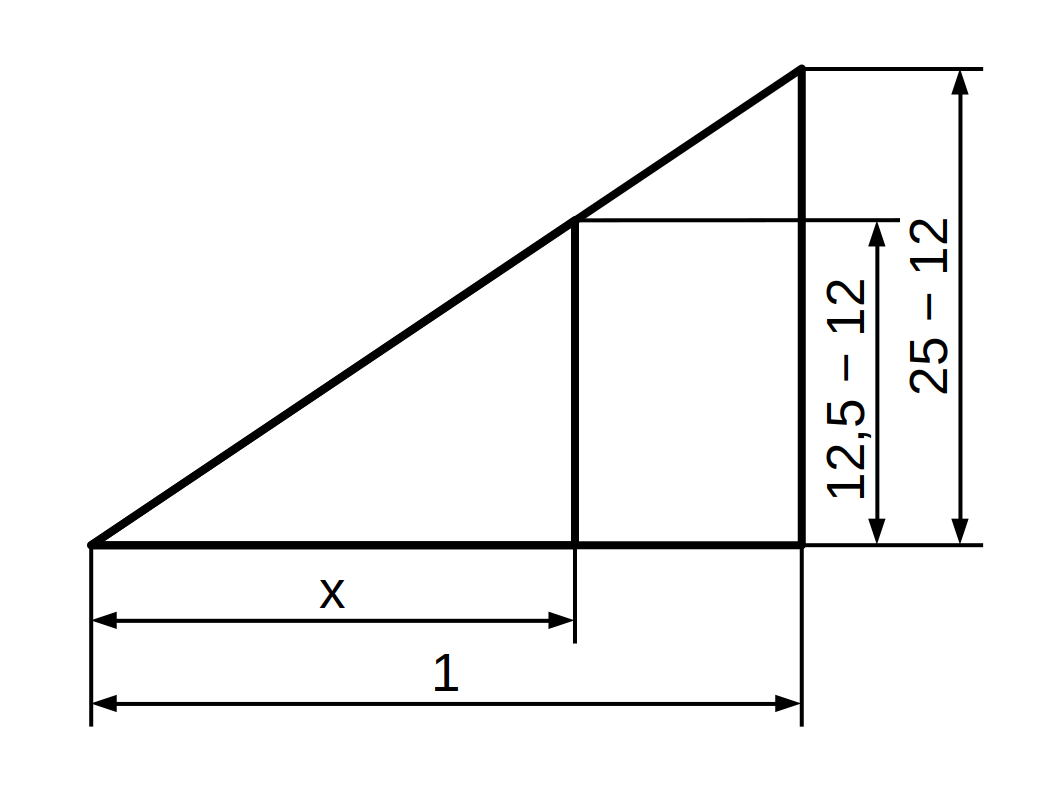
\includegraphics[width=4cm]{ej5_tr1.png} \\
\end{tabular}
{
\begin{tabular}{l}
$ \frac{x}{1}=\frac{0.5}{13} \rightarrow x = 0.0384 \Rightarrow Q_{1}^{(1)}= 1.0384 $
\end{tabular}}

\hspace*{1.1 cm}
\begin{tabular}{c}
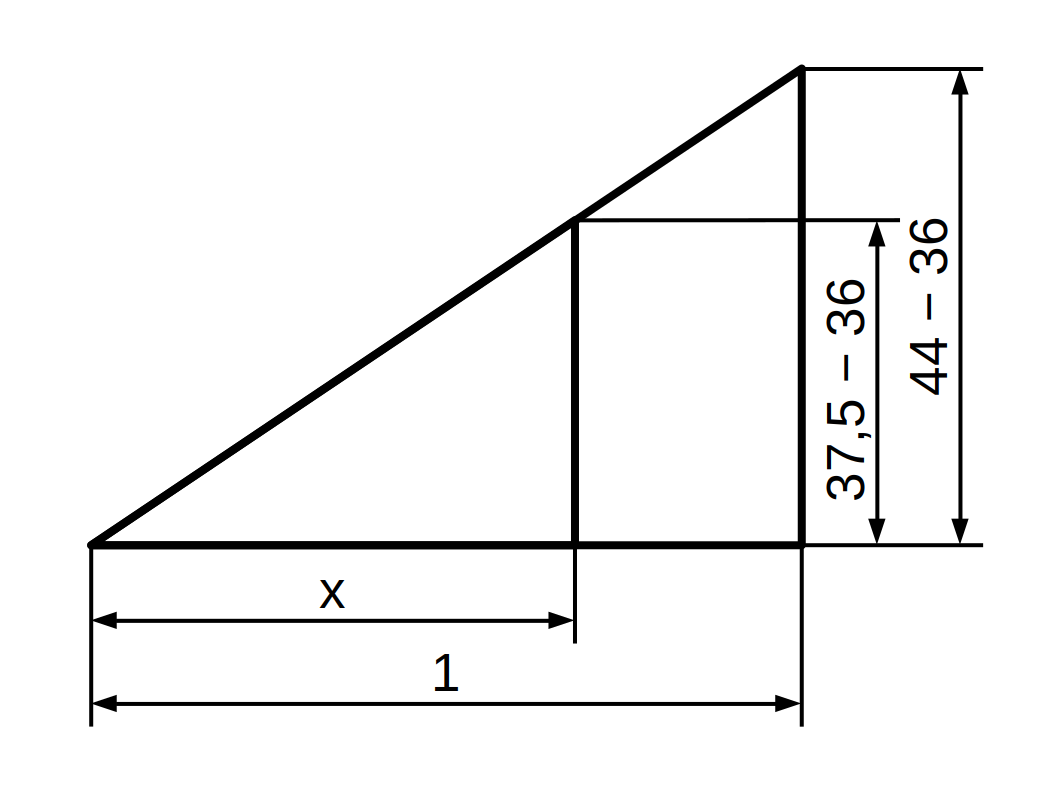
\includegraphics[width=4cm]{ej5_tr2.png} \\
\end{tabular}
{
\begin{tabular}{l}
$ \frac{x}{1}=\frac{1.5}{8} \rightarrow x = 0.1875 \Rightarrow Q_{3}^{(1)}= 3.1875 $
\end{tabular}}

\end{table}

Ya que $n^{(2)} / 4 = 7$, que es la cota superior de $I_2$, $Q_{1}^{(2)}= 3$.

\begin{table}[!htbp]
\hspace*{1.1 cm}
\begin{tabular}{c}
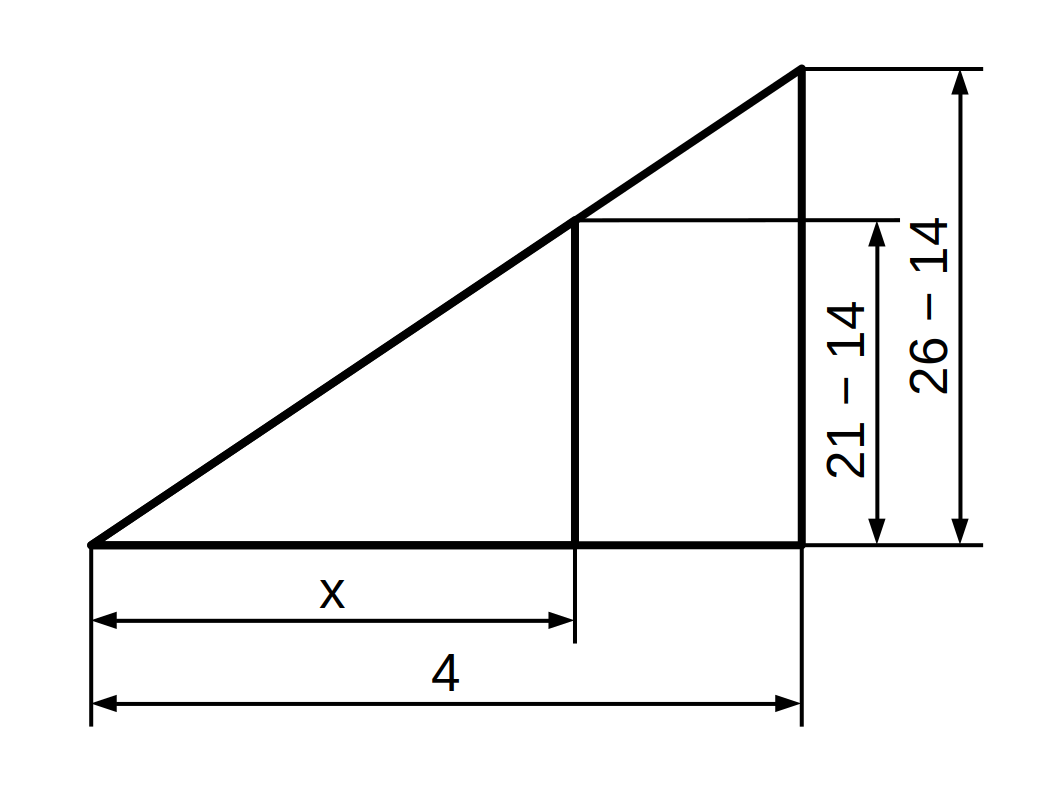
\includegraphics[width=4cm]{ej5_tr3.png} \\
\end{tabular}
{
\begin{tabular}{l}
$ \frac{x}{4}=\frac{7}{12} \rightarrow x = 2.\bar{3} \Rightarrow Q_{3}^{(2)}= 8.\bar{3} $
\end{tabular}}

\end{table}
			
		Por tanto, los recorridos son:
		\begin{itemize}
			\item[\textbf{(1)}] $R_I^{(1)} = Q_3^{(1)} - Q_1^{(1)} = 3.1875 - 1.0384 = 2.1491 $
			\item[\textbf{(2)}] $R_I^{(2)} = Q_3^{(2)} - Q_1^{(2)} = 8.\bar{3} -3 = 5.\bar{3}$
		\end{itemize}
		\emph{Interpretación: la longitud del intervalo en el que está incluido el 50\% central de los datos es de $2.1491$ y $5.\bar{3}$, respectivamente.}
\end{itemize}
\hspace{1cm} \\
\small {\textbf {Nota:} hemos realizado los cálculos suponiendo que la distribución es uniforme.} 
		\pagebreak
\begin{itemize}
		\item \textbf{Desviación típica:}
		\begin{itemize}
			\item[\textbf{(1)}] $$ \sigma^{(1)} = \sqrt[\leftroot{-2}\uproot{2}{}]{\frac{1}{n^{(1)}}  \sum_{i=1}^{k}c_i^2n_i^{(1)} - \left( \frac{1}{n^{(1)}}\sum_{i=1}^{k}c_{i}n_{i}^{(1)} \right)^2} = \sqrt[\leftroot{-2}\uproot{2}{}]{\frac{320.5}{50}-\frac{108^2}{50^2}} = 1.32 $$
			\item[\textbf{(2)}] $$ \sigma^{(2)} = \sqrt[\leftroot{-2}\uproot{2}{}]{\frac{1}{n^{(2)}}  \sum_{i=1}^{k}c_i^2n_i^{(2)} - \left( \frac{1}{n^{(2)}}\sum_{i=1}^{k}c_{i}n_{i}^{(2)} \right)^2} = \sqrt[\leftroot{-2}\uproot{2}{}]{\frac{1176}{28}-\frac{162^2}{28^2}} = 2.92 $$
		\end{itemize}
		\emph{Interpretación: para ver qué distribución es más homogénea, calculamos el \textbf{coeficiente de variación de Pearson}:}
		$$ C.V.(X^{(1)}) = \frac{\sigma_x^{(1)}}{|\bar{x}^{(1)}|} = \frac{1.32}{2.16} = 0.61 \hspace{1cm} C.V.(X^{(2)}) = \frac{\sigma_x^{(2)}}{|\bar{x}^{(2)}|} = \frac{2.92}{5.79} = 0.50 $$
		\emph{Vemos que la primera distribución está más dispersa.}
	\end{itemize}
\end{itemize}


%				##############################
%				#							 #
%				#  PROBLEMA 6				 #
%				#							 #
%				##############################


\pagebreak

\begin{itemize}
	\item[\textbf{6.}] Un móvil efectúa un recorrido de 100km en dos sentidos. En uno va a una velocidad constante de $v_1$ = 60km/h y el otro va a una velocidad constante de $v_2$ = 70km/h. Calcular la velocidad media del recorrido.
\end{itemize}

{\color{grey}\hrulefill}

\emph{Solución:}

\begin{enumerate}[label=\emph{\alph*})]
	\item[$\circledast$] \textbf{Población:} los móviles que efectúan el recorrido ($n=2$). \\ \textbf{Variable estadística:} la velocidad de cada móvil.
\end{enumerate}

Para resolver este problema, simplemente hemos de tener en cuenta la fórmula de la velocidad:

$$ v\hspace{0.1cm}\text{(velocidad)} = \frac{d\hspace{0.1cm}\text{(distancia)}}{t\hspace{0.1cm}\text{(tiempo)}} $$

Por tanto, para calcular la velocidad media del recorrido, $v_m$, tendremos que aplicar la fórmula:

$$ v_m\hspace{0.1cm}\text{(velocidad media)} = \frac{d_{\text{total}}\hspace{0.1cm}\text{(distancia total recorrida)}}{t_{\text{total}}\hspace{0.1cm}\text{(tiempo total empleado)}} $$

\begin{enumerate}
	\item Distancia total recorrida: \\
	$$ d_{\text{total}} = d_1 + d_2 = 100 \text{km} + 100 \text{km} = 200 \text{km} $$
	\item Tiempo total empleado: \\
	$$ t_{\text{total}} = t_1 + t_2 = \frac{d_1}{v_1} + \frac{d_2}{v_2} = \frac{100 \text{km}}{60 \text{km/h}} + \frac{100 \text{km}}{70 \text{km/h}} = 1.67 \text{h} + 1.43 \text{h} = 3.10 \text{h} $$
	\item Velocidad media:
	$$ v_m = \frac{d_{\text{total}}}{t_{\text{total}}} = \frac{d_1+d_2}{t_1+t_2} = \frac{200 \text{km}}{3.10 \text{h}} = 64.62\text{km/h} $$
\end{enumerate}

Por tanto, la velocidad media del recorrido es de $64.62$km/h. \\

Por otra parte, podríamos haber realizado la media armónica, dando el mismo resultado:
$$ v_m = \frac{2}{\frac{1}{v_1} + \frac{1}{v_2}} = \frac{2}{\frac{1}{60\text{km/h}} + \frac{1}{70\text{km/h}}} = 64.62\text{km/h}$$


%				##############################
%				#							 #
%				#  PROBLEMA 7				 #
%				#							 #
%				##############################


\pagebreak

\begin{itemize}
	\item[\textbf{7.}] Las acciones de una empresa han producido los siguientes rendimientos netos anuales:

% TABLA CON TEXTO A LA DERECHA (inicio)

\begin{table}[!htbp]
\hspace{5.7cm}
\begin{tabular}{cc}

Año & Rentabilidad \\ \hline
1994 & 12 \% \\
1995 & 10 \% \\
1996 & 7 \% \\
1997 & 6 \% \\
1998 & 5 \% \\
\end{tabular}
\end{table}

Obtener el rendimiento neto medio en esos cinco años.
\end{itemize}

{\color{grey}\hrulefill}

\emph{Solución:}

\begin{itemize}
	\item[$\circledast$] \textbf{Población:} los años en los que una empresa ha obtenido beneficios. \\ \textbf{Variable estadística:} la rentabilidad de la empresa. \\
	\small{\textbf{Nota:} para poder considerar el \emph{puñetero asterisco}, las modalidades de la variable estadística deberían estar ordenadas de menor a mayor.}
\end{itemize}
\hspace{1cm} \\
El rendimiento de la empresa es un cálculo que se acumula a lo largo de los años. De este modo:

$$ c_1 = 1.12c_0 \hspace{1cm} c_2 = 1.1c_1 \hspace{1cm} c_3 = 1.07c_2 \hspace{1cm} c_4 = 1.06c_3 \hspace{1cm} c_5 = 1.05c_4 $$

Queremos obtener el rendimiento medio, en otras palabras, el $i$ que cumple que:

$$ c_0(1+i)^5 = c_5 = c_0*1,12*1,1*1,07*1,06*1,05 \hspace{4cm} $$
$$ \rightarrow \hspace{0.2cm} i-1=G= \sqrt[\leftroot{-2}\uproot{2}{5}]{1,12*1,1*1,07*1,06*1,05}- 1 = 1.08-1 = 0.08 $$
\\
Por tanto, el rendimiento neto medio es del $8\%$. Nótese que hemos hecho una \emph{media geométrica}.


%				##############################
%				#							 #
%				#  PROBLEMA 8				 #
%				#							 #
%				##############################


\pagebreak

\begin{itemize}
	\item[\textbf{8.}] Un profesor califica a sus alumnos según el criterio siguiente: 40\% de suspensos, 30\% de aprobados, 15\% notables, 10\% sobresalientes y 5\% de matrículas. Las notas obtenidas son las siguientes:

% TABLA CON TEXTO A LA DERECHA (inicio)

\begin{table}[!htbp]
\hspace{1.5cm}
\begin{tabular}{|c|c|c|c|c|c|c|c|c|c|}
\hline
(0, 1] & (1, 2] & (2, 3] & (3, 4] & (4, 5] & (5, 6] & (6, 7] & (7, 8] & (8, 9] & (9, 10] \\ \hline
34 & 74 & 56 & 81 & 94 & 70 & 41 & 28 & 16 & 4 \\ \hline
\end{tabular}
\end{table}
	Calcular las notas máximas para obtener cada una de las calificaciones.
\end{itemize}

{\color{grey}\hrulefill}

\emph{Solución:}

\begin{itemize}
	\item[$\circledast$] \textbf{Población:} los estudiantes de un profesor. \\ \textbf{Variable estadística:} la nota que ha sacado cada estudiante.
\end{itemize}

La tabla tipo 3 para este problema es:

\begin{table}[!htbp]
\hspace{1cm}
\begin{tabular}{|c|c|c|c|c|}
\multicolumn{1}{c|}{$I_i$} & $n_i$ & $N_i$ & $c_i$ & $a_i$ \\ \hline
$(0, 1]$	&	34	&	34	&	0.5	&	1 \\
$(1, 2]$	&	74	&	108	&	1.5	&	1 \\
$(2, 3]$	&	56	&	164	&	2.5	&	1 \\
$(3, 4]$	&	81	&	245	&	3.5	&	1 \\
$(4, 5]$	&	94	&	339	&	4.5	&	1 \\
$(5, 6]$	&	70	&	409	&	5.5	&	1 \\
$(6, 7]$	&	41	&	450	&	6.5	&	1 \\
$(7, 8]$	&	28	&	478	&	7.5	&	1 \\
$(8, 9]$	&	16	&	494	&	8.5	&	1 \\
$(9, 10]$	&	4	&	498	&	9.5	&	1 \\ \hline
\multicolumn{1}{c}{} & \multicolumn{1}{|c|}{498} \\ \cline{2-2}
\end{tabular}
\end{table}

Para poder calcular las notas máximas para obtener cada una de las calificaciones, utilizaremos el concepto de \emph{percentil}:

\begin{itemize}
	\item \textbf{Suspenso:} bastará calcular el percentil 40, $P_{40}$. Esa será la nota máxima de los que han suspendido.
	\begin{table}[!htbp]
\hspace*{1.1 cm}
\begin{tabular}{c}
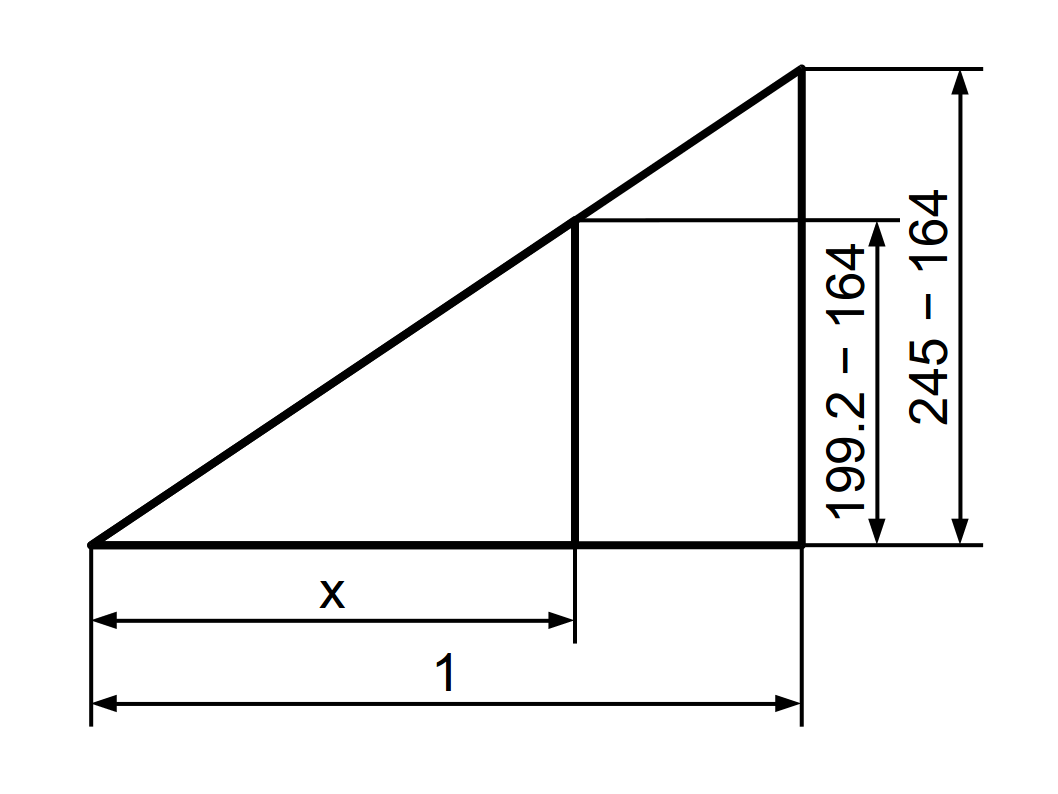
\includegraphics[width=4cm]{ej8_tr1.png} \\
\end{tabular}
{
\begin{tabular}{l}
$ \frac{x}{1}=\frac{35.2}{81} \rightarrow x = 0.4345 \Rightarrow P_{40}= 3.4345 $
\end{tabular}}

\end{table}	

\item \textbf{Aprobado:} bastará calcular el percentil 70, $P_{70}$. Esa será la nota máxima de los que tienen un aprobado.
	\begin{table}[!htbp]
\hspace*{1.1 cm}
\begin{tabular}{c}
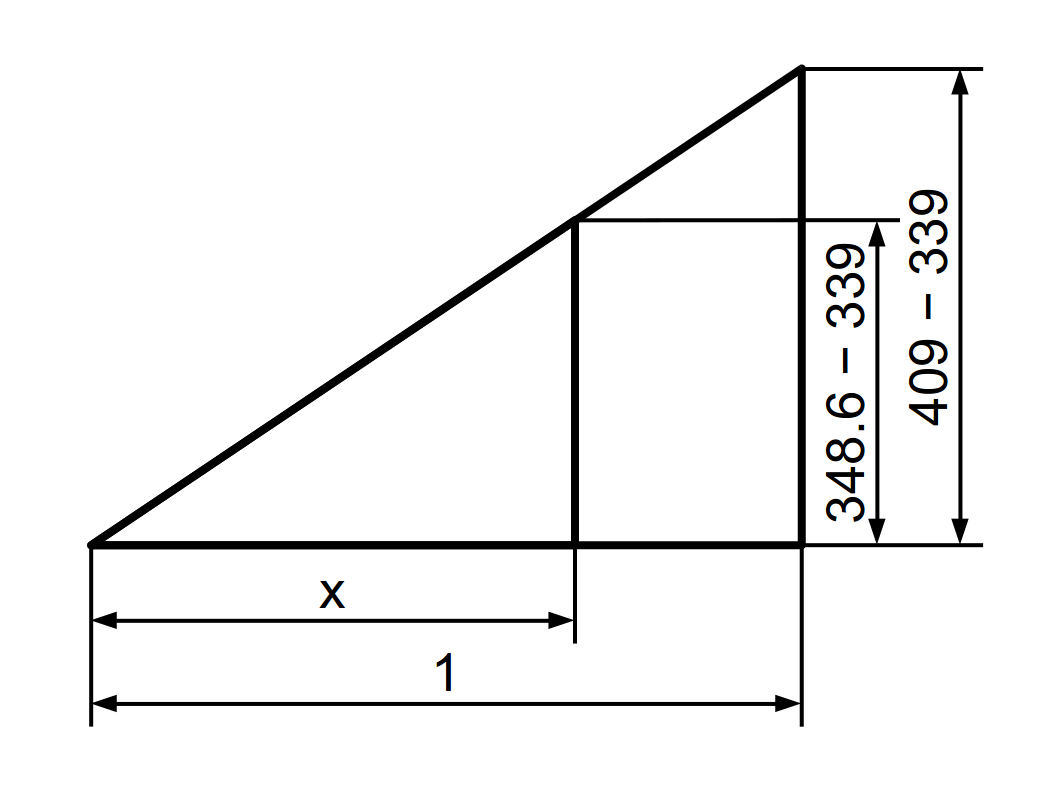
\includegraphics[width=4cm]{ej8_tr2.png} \\
\end{tabular}
{
\begin{tabular}{l}
$ \frac{x}{1}=\frac{9.6}{70} \rightarrow x = 0.1371 \Rightarrow P_{70}= 5.1371 $
\end{tabular}}

\end{table}

\pagebreak

\item \textbf{Notable:} bastará calcular el percentil 85, $P_{85}$. Esa será la nota máxima de los que tienen un notable.
	\begin{table}[!htbp]
\hspace*{1.1 cm}
\begin{tabular}{c}
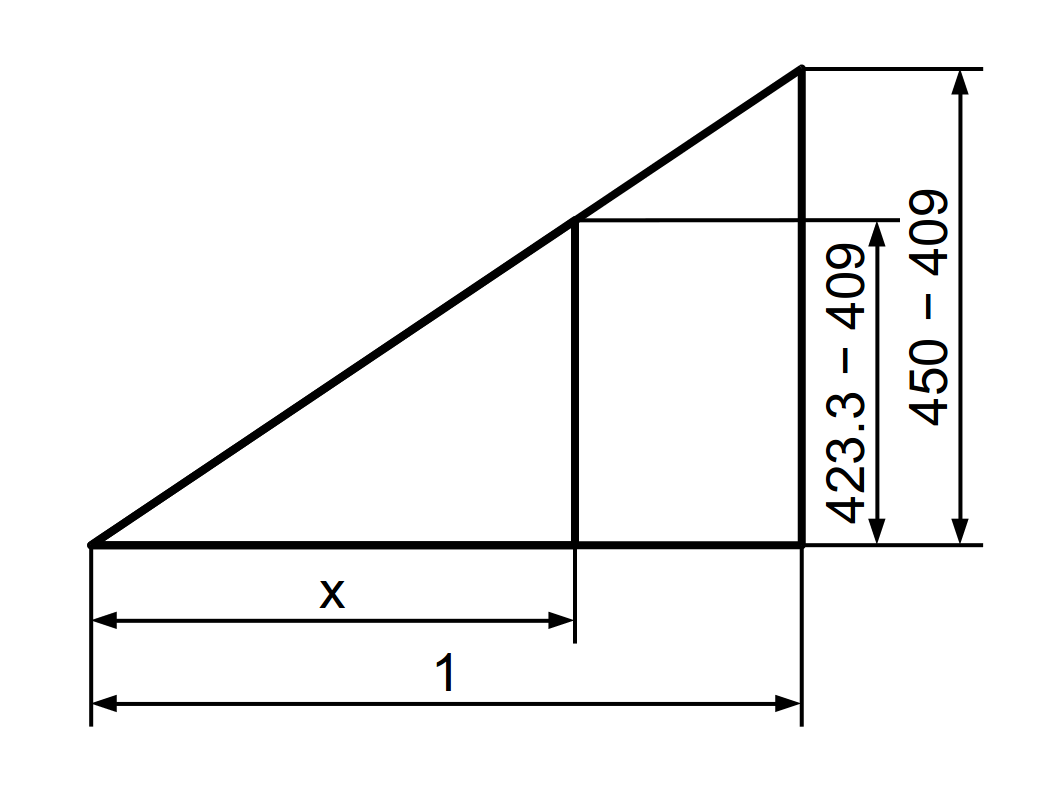
\includegraphics[width=4cm]{ej8_tr3.png} \\
\end{tabular}
{
\begin{tabular}{l}
$ \frac{x}{1}=\frac{14.3}{41} \rightarrow x = 0.3487 \Rightarrow P_{85}= 6.3487 $
\end{tabular}}

\end{table}

\item \textbf{Sobresaliente:} bastará calcular el percentil 95, $P_{95}$. Esa será la nota máxima de los que tienen un notable.
	\begin{table}[!htbp]
\hspace*{1.1 cm}
\begin{tabular}{c}
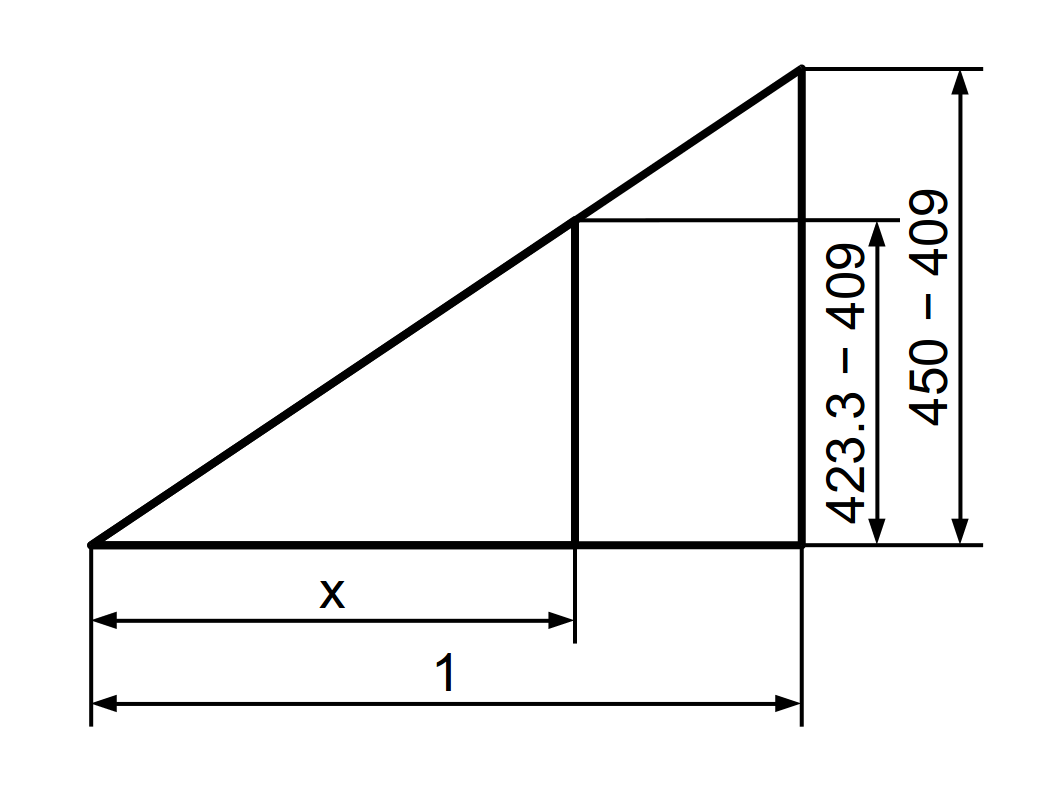
\includegraphics[width=4cm]{ej8_tr3.png} \\
\end{tabular}
{
\begin{tabular}{l}
$ \frac{x}{1}=\frac{23.1}{28} \rightarrow x = 0.825 \Rightarrow P_{95}= 7.825 $
\end{tabular}}

\end{table}

\item \textbf{Matrícula:} la nota máxima será un 10, puesto que es la cota superior del último intervalo.
	
\end{itemize}

\hspace{1cm} \\
\small {\textbf {Nota:} hemos realizado los cálculos suponiendo que la distribución es uniforme.} 

%				##############################
%				#							 #
%				#  PROBLEMA 9				 #
%				#							 #
%				##############################


\pagebreak

\begin{itemize}
	\item[\textbf{9.}] Se ha medido la altura de 110 jóvenes, obteniendo:

% TABLA CON TEXTO A LA DERECHA (inicio)

\begin{table}[!htbp]
\hspace{1.2cm}
\begin{tabular}{|c|c|c|c|c|c|}
\hline
Altura & ($1.55$, $1.60$] & ($1.60$, $1.70$] & ($1.70$, $1.80$] & ($1.80$, $1.90$] & ($1.90$, $2.00$] \\ \hline
Nº jóvenes & 18 & 31 & 24 & 20 & 17 \\ \hline
\end{tabular}
\end{table}
	\begin{enumerate}[label=\emph{\alph*})]
		\item Si se consideran bajos el 3\% de los individuos de menor altura, ¿cuál es la altura máxima que pueden alcanzar?
		\item Si se consideran altos el 18\% de los individuos de mayor altura, ¿cuál es su altura mínima?
		\item ¿Qué altura es superada sólo por 1/4 de los jóvenes?
		\item Calcular el número de jóvenes cuya altura es superior a $1.75$
		\item Calcular la altura máxima de los 11 jóvenes más bajos.
		\item Calcular la altura mínima de los 11 jóvenes más altos.
	\end{enumerate}
\end{itemize}

{\color{grey}\hrulefill}

\emph{Solución:}

\begin{enumerate}[label=\emph{\alph*})]
	\item Bastaría calcular el percentil $P_3$, pues el 3\% estará por debajo de éste.


%% AQUIII

\begin{table}[!htbp]
\hspace*{1.1 cm}
\begin{tabular}{c}
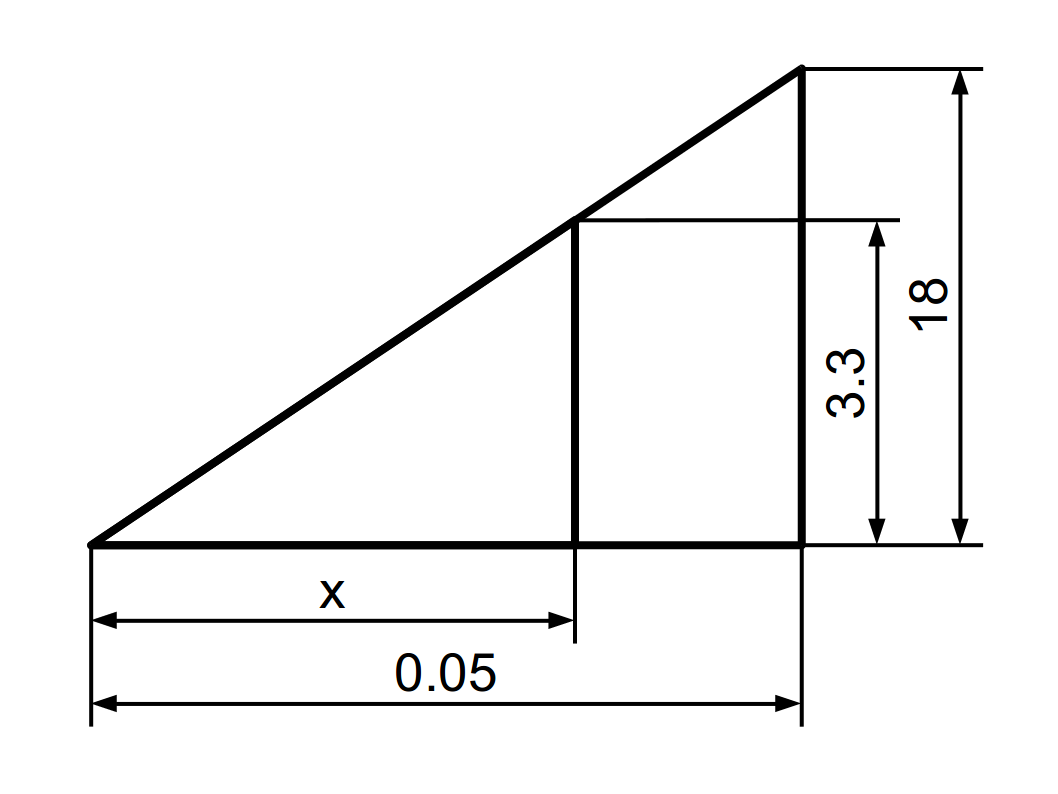
\includegraphics[width=4cm]{ej9_tr1.png} \\
\end{tabular}
{
\begin{tabular}{l}
$ \frac{x}{3.3}=\frac{0.05}{18} \rightarrow x = 0.009 \Rightarrow P_3 = 1.559 $
\end{tabular}}

\end{table}


	\item Bastaría calcular el percentil $P_{82}$, pues el 18\% estará por encima de éste.

\begin{table}[!htbp]
\hspace*{1.1 cm}
\begin{tabular}{c}
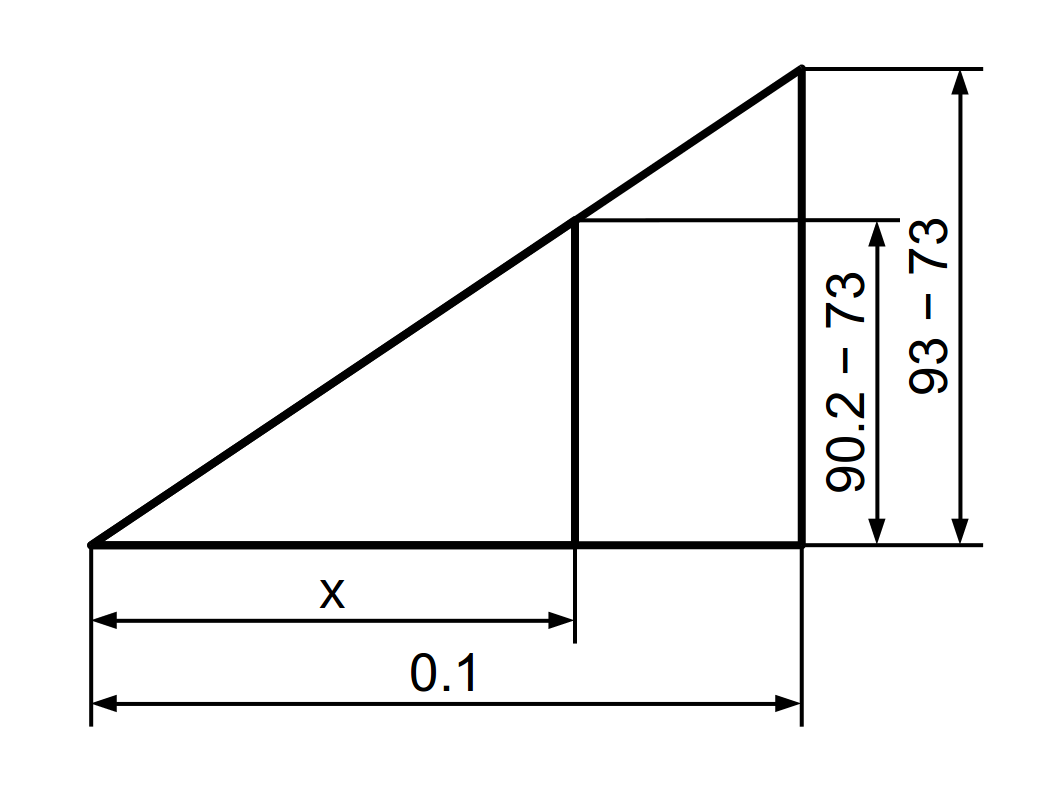
\includegraphics[width=4cm]{ej9_tr2.png} \\
\end{tabular}
{
\begin{tabular}{l}
$ \frac{x}{17.2}=\frac{0.1}{20} \rightarrow x = 0.086 \Rightarrow P_{82} = 1.886 $
\end{tabular}}

\end{table}

	\item Bastaría calcular el percentil $P_{75}$, pues el 25\% estará por encima de éste.
\begin{table}[!htbp]
\hspace*{1.1 cm}
\begin{tabular}{c}
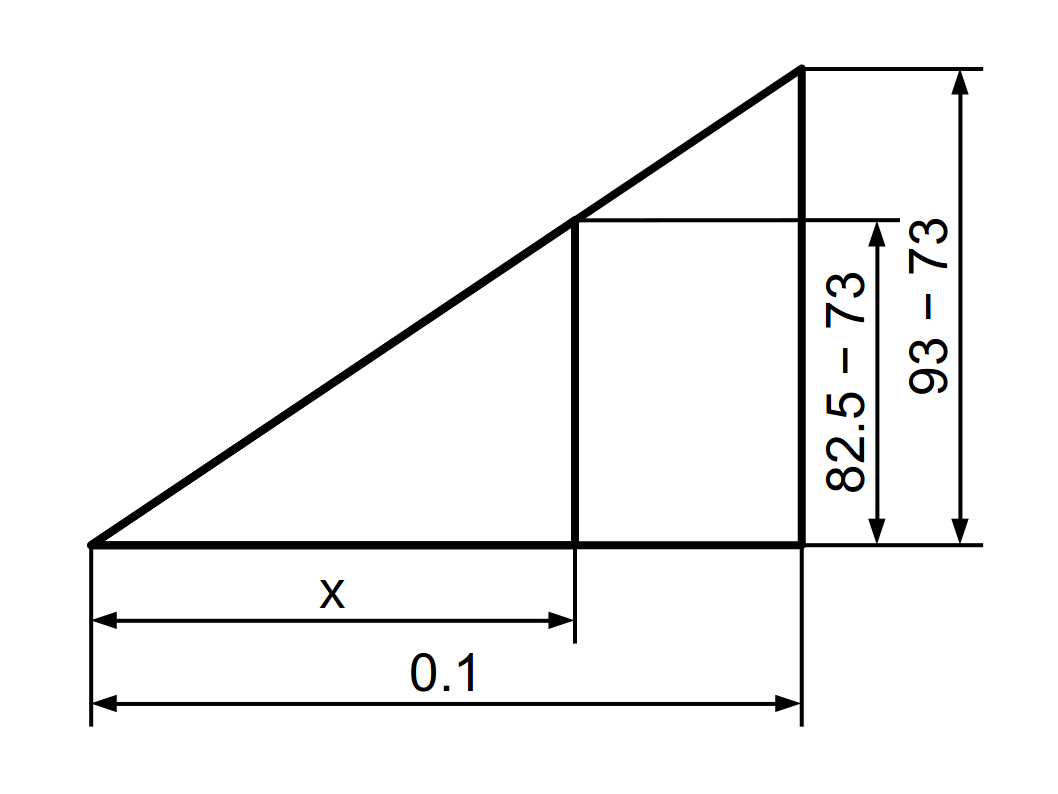
\includegraphics[width=4cm]{ej9_tr3.png} \\
\end{tabular}
{
\begin{tabular}{l}
$ \frac{x}{9.5}=\frac{0.1}{20} \rightarrow x = 0.0475 \Rightarrow P_{75} = 1.8475 $
\end{tabular}}

\end{table}
	
	\pagebreak
	\item Tomamos el intervalo donde se encuentra el $1.75$, $I_3 = (1.70, 1.80]$, y suponiendo que la distribución es homogénea, calculamos el valor correspondiente dentro de la función de distribución. 

\begin{table}[!htbp]
\hspace*{1.1 cm}
\begin{tabular}{c}
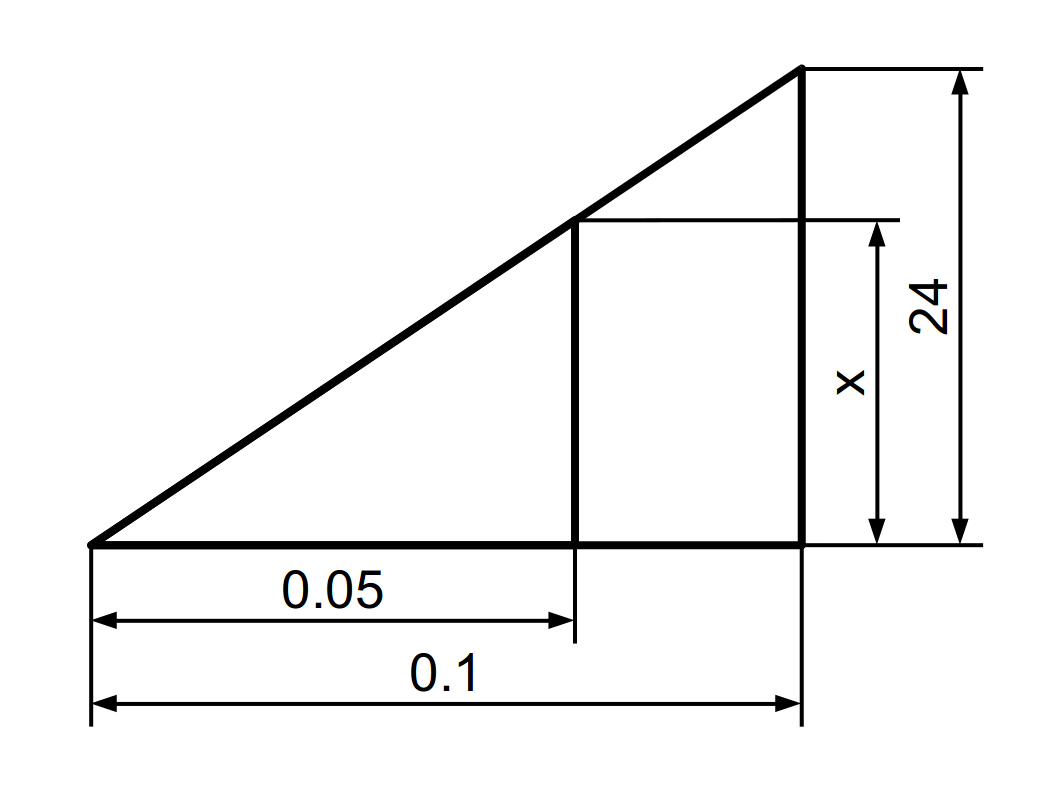
\includegraphics[width=4cm]{ej9_tr4.png} \\
\end{tabular}
{
\begin{tabular}{l}
$ \frac{x}{24}=\frac{0.05}{0.1} \rightarrow x = 12 $
\end{tabular}}
\end{table}

	\item Tomamos el intervalo donde se encuentra el joven número 11 si los ordenamos de menor a mayor altura, es decir, el intervalo $I_1 = (1.55,1.60]$, y suponiendo que la distribución es homogénea, calculamos el valor correspondiente dentro de la función de distribución. 

\begin{table}[!htbp]
\hspace*{1.1 cm}
\begin{tabular}{c}
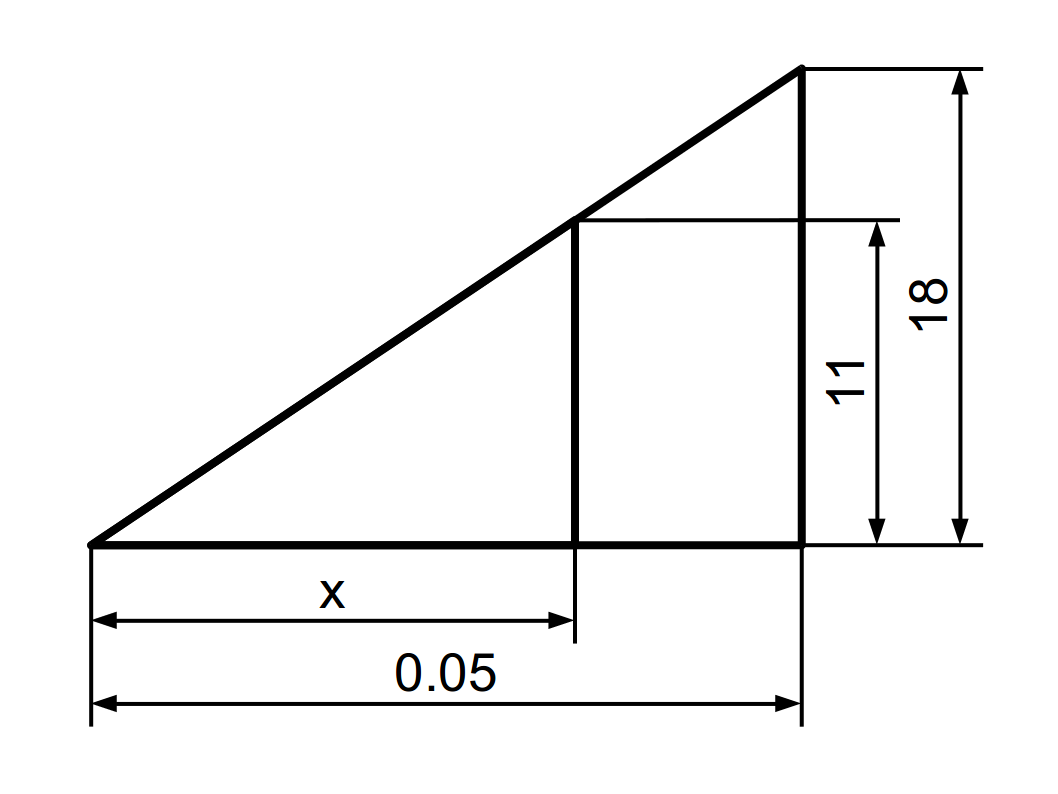
\includegraphics[width=4cm]{ej9_tr5.png} \\
\end{tabular}
{
\begin{tabular}{l}
$ \frac{x}{0.05}=\frac{11}{18} \rightarrow x = 0.0305 \Rightarrow \text{Altura}_{11} = 1.5805 $

\end{tabular}}
\end{table}

	\item Tomamos el intervalo donde se encuentra el joven número 99 si los ordenamos de menor a mayor altura, es decir, el joven número 6 en el intervalo $I_5 = (1.90,2.00]$, y suponiendo que la distribución es homogénea, calculamos el valor correspondiente dentro de la función de distribución. 

\begin{table}[!htbp]
\hspace*{1.1 cm}
\begin{tabular}{c}
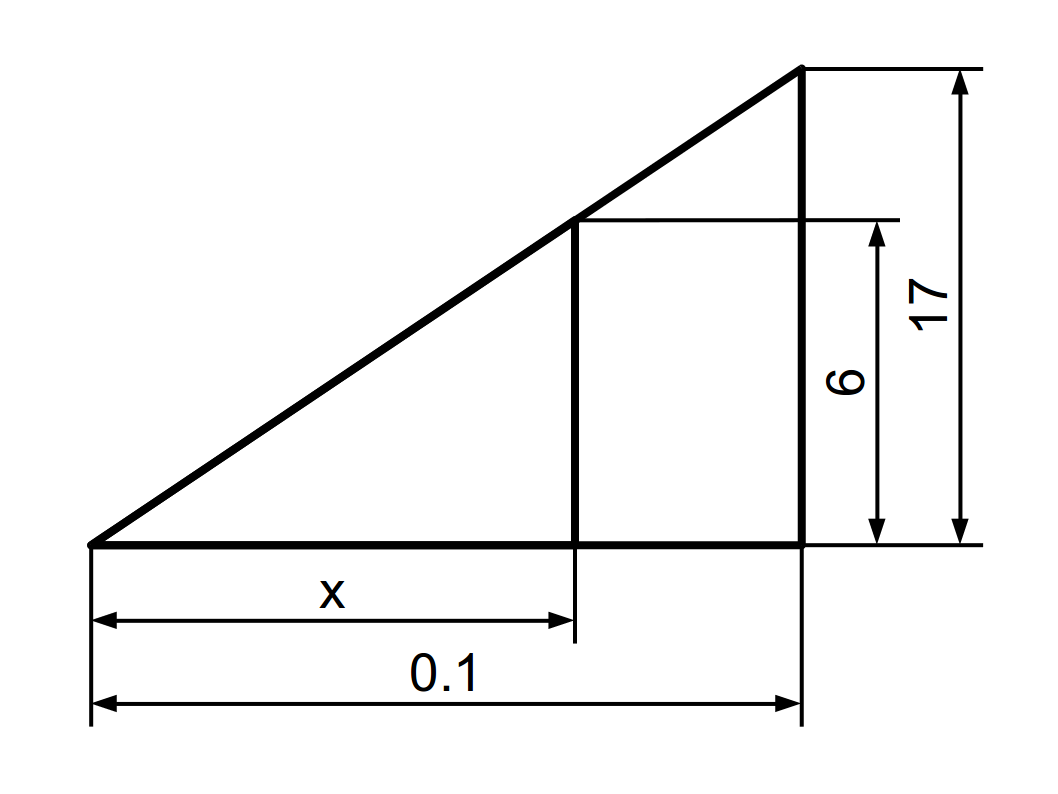
\includegraphics[width=4cm]{ej9_tr6.png} \\
\end{tabular}
{
\begin{tabular}{l}
$ \frac{x}{0.1}=\frac{6}{17} \rightarrow x = 0.03529 \Rightarrow \text{Altura}_{99} = 1.9353 $

\end{tabular}}
\end{table}
	\end{enumerate}

\hspace{1cm} \\
\small {\textbf {Nota:} hemos realizado los cálculos suponiendo que la distribución es uniforme.} 

%				##############################
%				#							 #
%				#  PROBLEMA 10				 #
%				#							 #
%				##############################


\pagebreak

\begin{itemize}
	\item[\textbf{10.}] Realizando una prueba para el estudio del cáncer a 150 personas se obtuvo la siguiente tabla según la edad de los enfermos:

% TABLA CON TEXTO A LA DERECHA (inicio)

\begin{table}[!htbp]
\hspace{2.7cm}
\begin{tabular}{|c|c|c|c|c|c|}
\hline
Edad & (10, 30] & (30, 40] & (40, 50] & (50, 60] & (60, 90] \\ \hline
Nº enfermos & 15 & 22 & 48 & 40 & 25 \\ \hline
\end{tabular}
\end{table}
	\begin{enumerate}[label=\emph{\alph*})]
		\item Calcular la edad más común de los individuos estudiados.
		\item Calcular la edad mínima y máxima del 30\% central de los individuos.
		\item Calcular el recorrido intercuartílico y la desviación típica.
		\item Calcular e interpretar los valores de los coeficientes de asimetría y curtosis.
	\end{enumerate}
\end{itemize}

{\color{grey}\hrulefill}

\emph{Solución:} \\ 

La tabla completa de este problema es:

\begin{table}[!htbp]
\hspace{1cm}\begin{tabular}{|c|c|c|c|c|c|c|c|c|}
\multicolumn{1}{c|}{$I_i$} & $n_i$ & $N_i$ & $f_i$ & $c_i$ & $c_in_i$ & $c_i^2n_i$ & $a_i$ & $h_i$ \\ \hline
$[10, 30]$ & 15 & 15 & 0.1 & 20 & 300 & 6000 & 20 & 0.75 \\
$(30, 40]$ & 22 & 37 & 0.147 & 35 & 770 & 26950 & 10 & 2.2 \\
$(40, 50]$ & 48 & 85 & 0.32 & 45 & 2160 & 97200 & 10 & 4.8 \\
$(50, 60]$ & 40 & 125 & 0.267 & 55 & 2200 & 121000 & 10 & 4 \\
$(60, 90]$ & 25 & 150 & 0.167 & 75 & 1875 & 140625 & 30 & 0.833 \\
\hline
\multicolumn{1}{c}{} & \multicolumn{1}{|c|}{150} & \multicolumn{1}{c}{} & \multicolumn{1}{|c|}{$\approx1$} &\multicolumn{1}{c}{} &\multicolumn{1}{|c|}{7305}& \multicolumn{1}{c|}{391775}  \\ \cline{2-2} \cline{4-4} \cline{6-7}
\end{tabular}
\end{table}

\begin{enumerate}[label=\emph{\alph*})]
	\item Calcularemos la moda. Para ello, aplicamos el \emph{teorema de Tales} sobre el histograma y obtenemos la siguiente proporción: 


\begin{table}[!htbp]
\hspace*{1.1 cm}
\begin{tabular}{c}
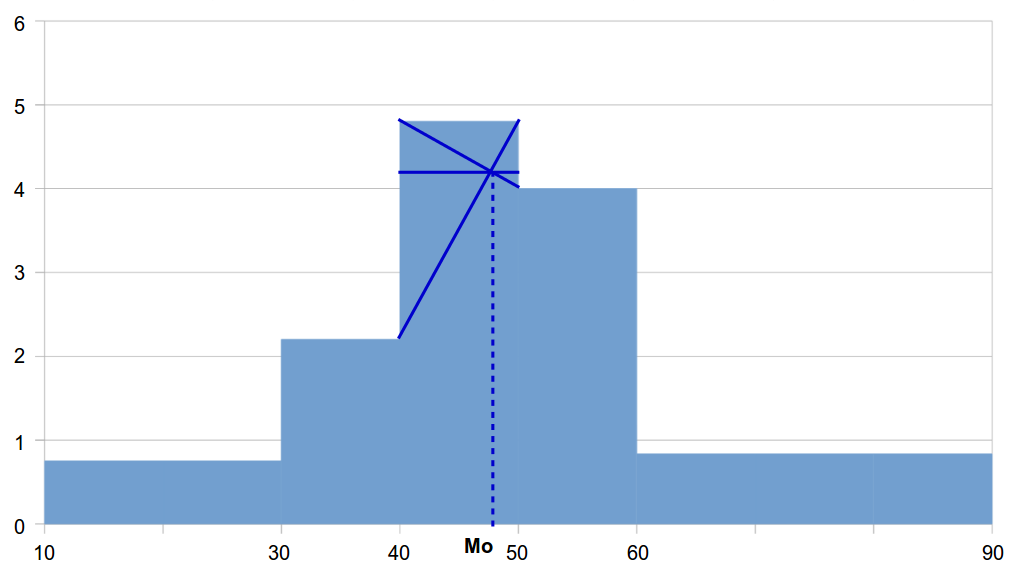
\includegraphics[width=8cm]{ej10_hist.png} \\
\end{tabular}
{
\begin{tabular}{l}
$ \frac{0.5}{0.5+2.\bar{6}} = \frac{Mo-40}{10} \Rightarrow Mo = 41.5789$
\end{tabular}}

\end{table}

\pagebreak
	\item Calcularemos el percentil 35, $P_{35}$, y el percentil 65, $P_{65}$.

\begin{table}[!htbp]
\hspace*{1.1 cm}
\begin{tabular}{c}
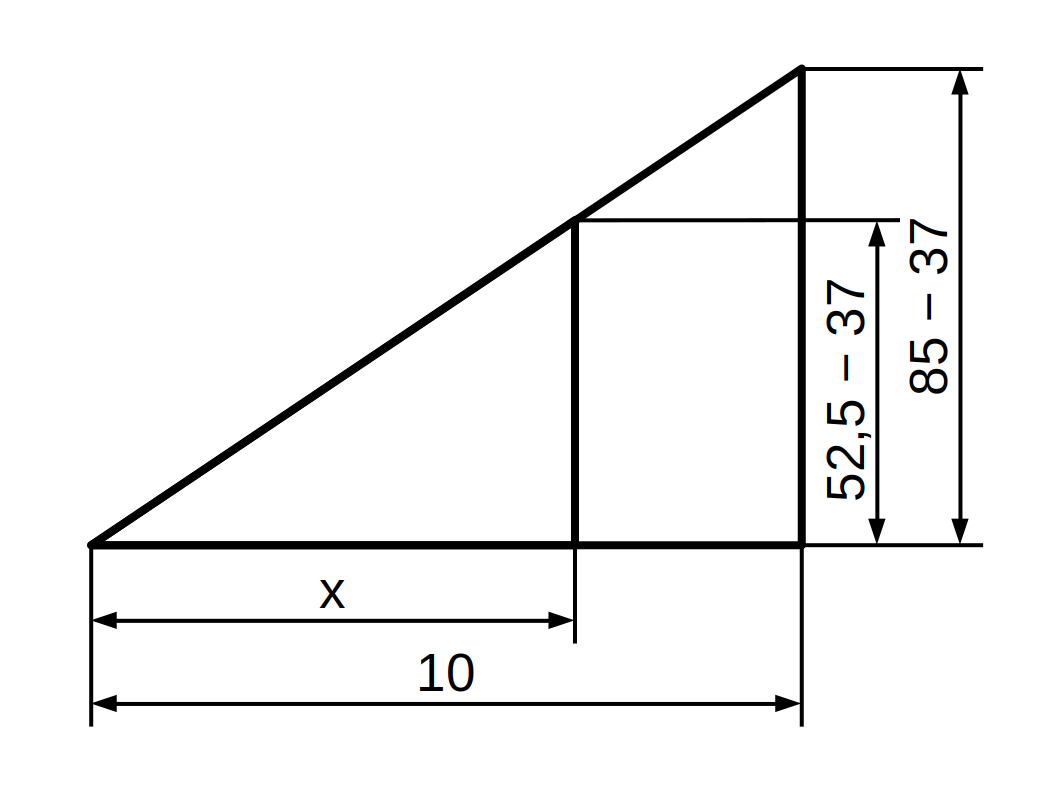
\includegraphics[width=4cm]{ej10_tr1.png} \\
\end{tabular}
{
\begin{tabular}{l}
$ \frac{x}{15.5}=\frac{10}{48} \rightarrow x = 3.229 \Rightarrow P_{35} = 43.229 $
\end{tabular}}

\hspace*{1.1 cm}
\begin{tabular}{c}
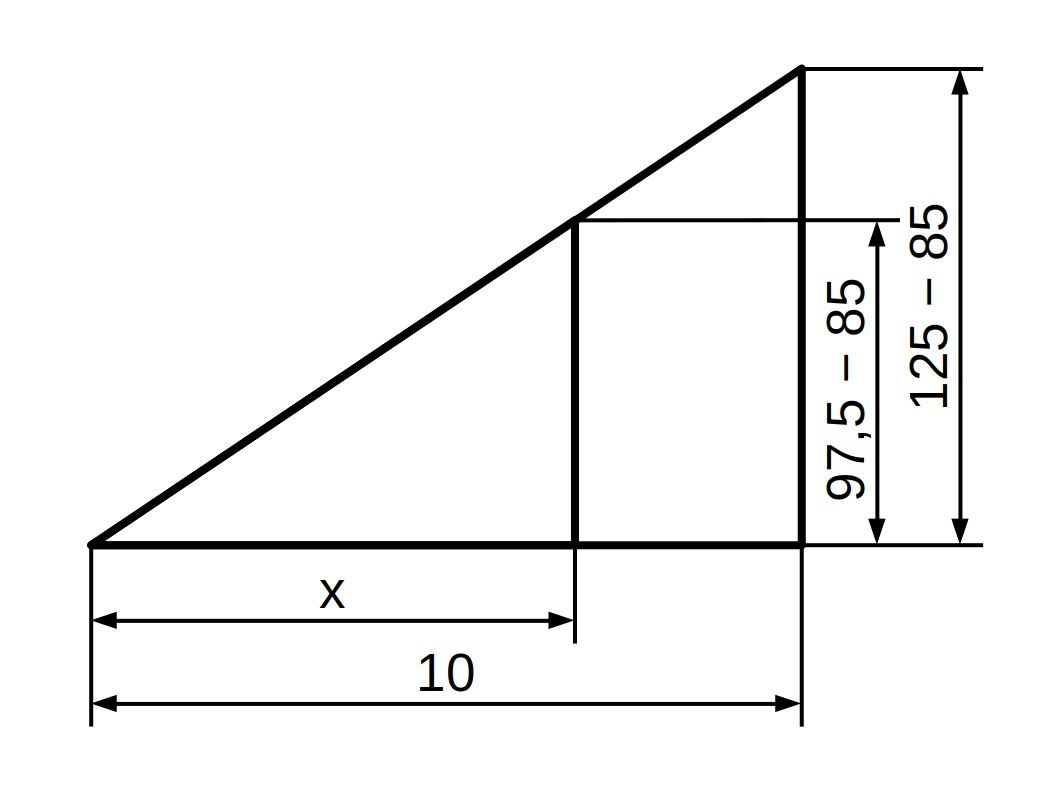
\includegraphics[width=4cm]{ej10_tr2.png} \\
\end{tabular}
{
\begin{tabular}{l}
$ \frac{x}{12.5}=\frac{10}{40} \rightarrow x = 3.125 \Rightarrow P_{65} = 53.125 $
\end{tabular}}

\end{table}
	\item[] \emph{La edad mínima del 30\% central de los individuos es de $43.229$ años (es decir, $43$ años), mientras que la máxima es de $53.125$ años (es decir, $54$ años).} \\
	\item Calcularemos los cuartiles, de forma análoga a problemas anteriores:
	\begin{table}[!htbp]
\hspace*{1.1 cm}
\begin{tabular}{c}
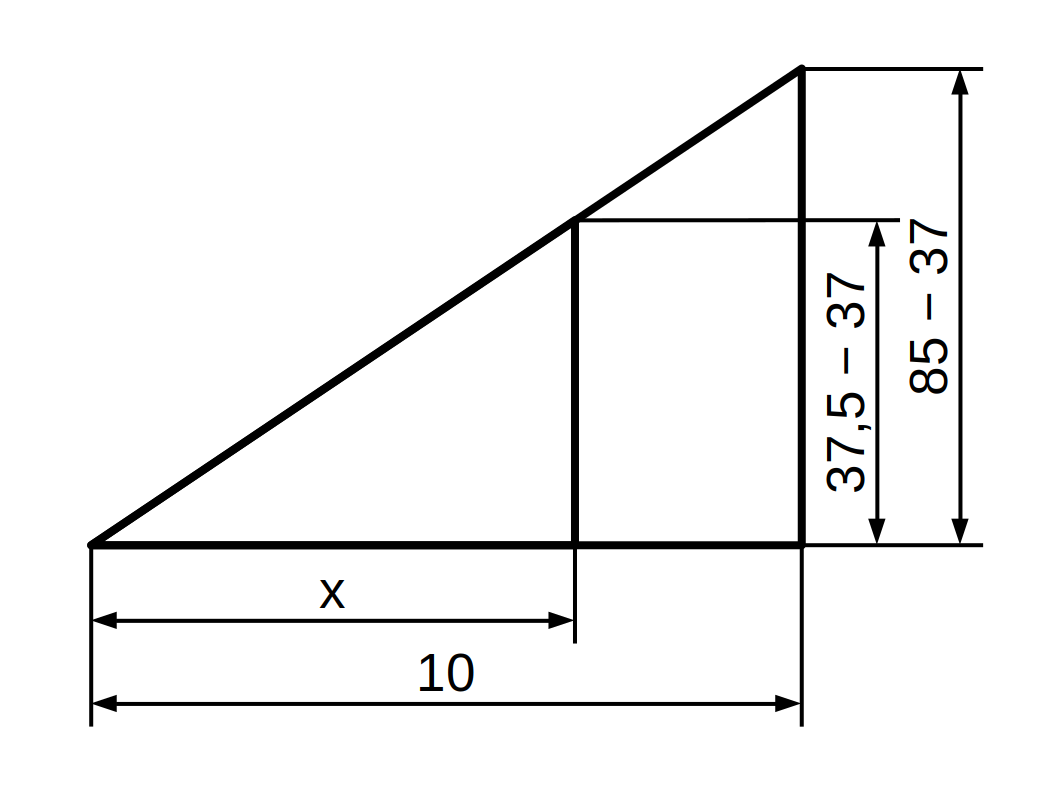
\includegraphics[width=4cm]{ej10_tr3.png} \\
\end{tabular}
{
\begin{tabular}{l}
$ \frac{x}{10}=\frac{0.5}{48} \rightarrow x = 0.1042 \Rightarrow Q_{1}= 40.1042 $
\end{tabular}}

\hspace*{1.1 cm}
\begin{tabular}{c}
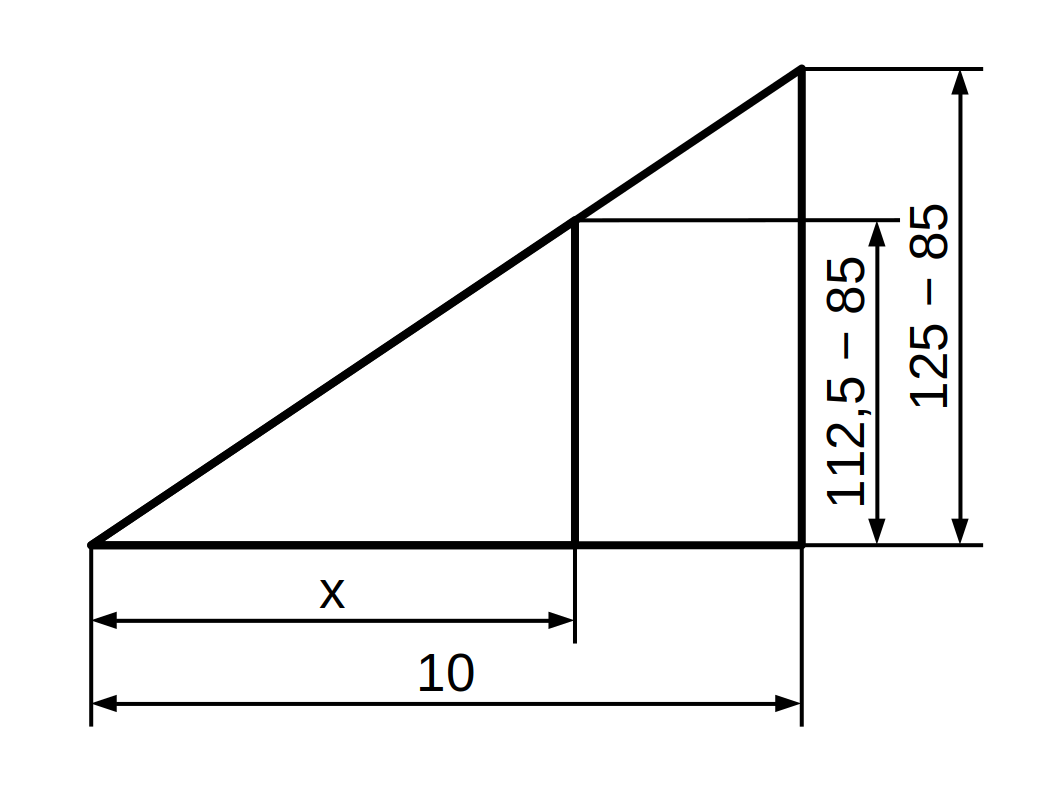
\includegraphics[width=4cm]{ej10_tr4.png} \\
\end{tabular}
{
\begin{tabular}{l}
$ \frac{x}{10}=\frac{27.5}{40} \rightarrow x = 6.875 \Rightarrow Q_{3}= 56.875 $
\end{tabular}}
\end{table}
\begin{itemize}
		\item \textbf{Recorrido intercuartílico:} $R_I = Q_3 - Q_1 = 56.875-40.1042 = 16.7708$. \\
		\emph{La longitud del intervalo en el que está incluido el 50\% central de los datos es de $16.7708$.}
		\item \textbf{Desviación típica:} lo calcularemos mediante el \emph{teorema de König}: 
		$$ \sigma = \sqrt[\leftroot{-2}\uproot{2}{}]{\frac{1}{n}  \sum_{i=1}^{k}c_i^2n_i - \left( \frac{1}{n}\sum_{i=1}^{k}c_{i}n_{i} \right)^2} = 15.496 $$
		
	\end{itemize}

\hspace{1cm} \\
\small {\textbf {Nota:} hemos realizado los cálculos suponiendo que la distribución es uniforme.} 
\pagebreak
	\item Calcularemos los coeficientes de asimetría y curtosis:
	
	\begin{itemize}
		\item \textbf{Coeficiente de asimetría:} lo calcularemos mediante el \emph{coeficiente de asimetría de Fisher:}
	
		$$ \gamma_1(X) = \frac{\mu^3}{\sigma_x^3} = \frac{1}{n} \sum_{i=1}^{k}{\left(\frac{c_i-\bar{x}}{\sigma_x}\right)^3 = -0.66} $$

Como $\gamma_1(X) < 0$, estamos ante una distribución \emph{asimétrica por la izquierda} o \emph{negativa}. \\

	\item \textbf{Coeficiente de curtosis:} lo calcularemos mediante el \emph{coeficiente de curtosis de Fisher:}
	$$ \gamma_2(X) = \frac{\mu^4}{\sigma_x^4} - 3 = \frac{1}{n} \sum_{i=1}^{k}{\left(\frac{c_i-\bar{x}}{\sigma_x}\right)^4 - 3 = -1.72} $$

Como $\gamma_2(X) < 0$, estamos ante una distribución \emph{platicúrtica}.
	\end{itemize}

	
\end{enumerate}

\end{document}